\documentclass[a4paper]{article}
\usepackage{geometry}
\geometry{
	a4paper,
	total={170mm,257mm},
	left=27mm,
	right=30mm,
	top=30mm,
	bottom= 30mm
}
\usepackage{lipsum}\usepackage{geometry}
\usepackage{tabu}
\usepackage{adjustbox}
\usepackage[english]{babel}
\usepackage[utf8]{inputenc}
\usepackage{longtable}
\usepackage{amsmath}
\usepackage[toc,page]{appendix}
\usepackage{hyperref}
\usepackage{graphicx}
\usepackage{enumitem}
\usepackage[colorinlistoftodos]{todonotes}
\usepackage{tikz}
\newcommand*\circled[1]{\tikz[baseline=(char.base)]{
		\node[shape=circle,draw,inner sep=0.5pt] (char) {#1};}}
\usetikzlibrary{fit,positioning}
\usepackage{authblk}
\usepackage[algo2e]{algorithm2e}
\usepackage{algorithmic}  
\usepackage{algorithm}
\usepackage{comment}
\usepackage{array,longtable,booktabs,siunitx}
\usepackage{array}% http://ctan.org/pkg/array
\usepackage{natbib}
\RequirePackage{natbib}
\makeatletter
\g@addto@macro{\endtabular}{\rowfont{}}% Clear row font
\makeatother
\newcommand{\rowfonttype}{}% Current row font
\newcommand{\rowfont}[1]{% Set current row font
	\gdef\rowfonttype{#1}#1%
}
\newcolumntype{L}{>{\rowfonttype}l}
\title{A Dynamic Additive and Multiplicative Effects Model\\
	with Application to the United Nations Voting Behaviors}
%\author{Bomin Kim}

\author[1]{Bomin Kim}
\author[1]{Xiaoyue Niu}
\author[1]{David Hunter}
\author[2]{Xun Cao}
\affil[1]{Department of Statistics, The Pennsylvania State University}
\affil[2]{Department of Political Science, The Pennsylvania State University}
\date{}
\begin{document}
	\maketitle
	\begin{abstract}
		\noindent  
		In this paper, we introduce a statistical regression model for discrete-time networks that are correlated over time. Our model is a dynamic version of a Gaussian additive and multiplicative effects (DAME) model which extends the latent factor network model of \cite{hoff2009multiplicative} and the additive and multiplicative effects model of \cite{minhas2016inferential}, by incorporating the temporal correlation structure into the prior specifications of the parameters. The temporal evolution of the network is modeled through a Gaussian process (GP) as in \cite{durante2013nonparametric}, where we estimate the unknown covariance structure from the dataset. We analyze the United Nations General Assembly voting data from 1983 to 2014 \citep{12379_2016} and show the effectiveness of our model at inferring the dyadic dependence structure among the international voting behaviors as well as allowing for a varying number of nodes over time. Overall, the DAME model shows significantly better fit to the dataset compared to the alternative approaches. Moreover, after controlling for other dyadic covariates such as geographic distances and bilateral trade between countries, the model-estimated additive effects, multiplicative effects, and their movements reveal interesting and meaningful foreign policy positions and alliances of various countries. 
	\end{abstract}
	\section{Introduction} \label{sec: Introduction}
	In recent decades, social network analysis has been well-established and is widely used in a variety of applications, ranging from friendship and collaboration networks to disease transmission.  Because a network naturally evolves over time, there has been a growing need for methods of modeling networks that change over time. A number of models have been suggested that are extensions of static network models, such as the temporal exponential random graph model (TERGM) \citep{hanneke2010discrete} and the dynamic stochastic blockmodel \citep{xu2013dynamic}, or new models for network dynamics, such as the stochastic actor oriented model (SAOM) \citep{snijders2010introduction}. On the other side, there are dynamic network models that give consideration to the unobserved latent space \citep{hoff2002latent}---the structure of the network that is not explained through the use of exogenous node and dyad covariates. To provide novel insights into the latter, we extend existing latent factor models \citep{hoff2005bilinear,hoff2009multiplicative,hoff2014amen,minhas2016inferential} and develop the dynamic additive and multiplicative effects model (DAME) for discrete-time networks, with emphasis on the latent structures---unmeasured attributes of nodes for tie formations and their changes over time.\\ \newline
 \cite{hoff2002latent} introduces a class of models where the probability of a relation between actors depends on the positions of individuals in an unobserved ``social space". There are two specifications in the latent space model: (i) ``the latent distance model" which is built upon the latent Euclidean space; and (ii) ``the latent factor model" which stems from the projection model. Specifically, there are several versions of the latent projection model in which the probability of a tie beteween nodes $i$ and $j$ is determined by inner product the two nodes' latent positions $f(\boldsymbol{v}_i, \boldsymbol{v}_j)={(\boldsymbol{v}_i'\boldsymbol{v}_j)}{|\boldsymbol{v}_j|^{-1}}$. \cite{hoff2005bilinear} proposes the symmetric multiplicative interaction effect ($\boldsymbol{v}_i^\prime \boldsymbol{v}_j$) into the network generalized linear model in order to capture third-order dependence patterns---often described by the three features, transitivity, balance, and clusterability. \cite{hoff2008modeling} parameterizes the multiplicative effects via eigendecomposition $\boldsymbol{u}_i^T\mathbf{\Lambda}\boldsymbol{u}_j$, and demonstrates that the latent eigenmodel is able to represent a wide array of patterns in the data due to its unrestricted low-rank approximation to the symmetric relational data. \cite{hoff2009multiplicative} extends the framework to model asymmetric social networks using the singular value decomposition $\boldsymbol{u}_i^T\mathbf{D}\boldsymbol{v}_j$. Finally, \cite{hoff2014amen} and \cite{minhas2016inferential} combine the additive and multiplicative effects to model the second-order (or reciprocity) and third-order dependencies and estabilish the AME---additive and multiplicative effects ---regression model for dyadic response data $y_{ij}$, in which 
	\begin{equation}\label{AME}
		\begin{aligned}
			&y_{ij} = g(\theta_{ij}),\\
			& \theta_{ij} = \boldsymbol{\beta}^T\mathbf{X}_{ij} + e_{ij}, \mbox{ and }\\
			& e_{ij} = a_i + b_j + \epsilon_{ij} + \alpha(\boldsymbol{u}_i, \boldsymbol{v}_j), 
		\end{aligned}
	\end{equation}
where $\alpha(\boldsymbol{u}_i, \boldsymbol{v}_j) = \boldsymbol{u}_i^T\mathbf{D}\boldsymbol{v}_j$ and $ g(\theta_{ij})$ is a link function used to model various types of relational matrices such as continuous, binary, ordinal, or rank-based responses.\\ \newline
As dynamic network analysis has become an emergent scientific field, there has been a growing number of dynamic network models that incorporate the latent space models in the last decade \citep{kim2017review}. For instance, latent distance models have been a strong motivation for various dynamic network models by many authors \citep{sarkar2005dynamic,sarkar2007latent,sewell2015latent,sewell2016latent,friel2016interlocking}, providing ample references for the reader interested in these specific problems. On the other hand, a comparatively small literature employs the AME framework to develop dynamic network models. \cite{ward2007persistent} first introduces the concept of dynamic latent factors, and this idea is expanded by \cite{ward2013gravity} to analyze bilateral trade using the generalized bi-linear mixed effect model \citep{hoff2005bilinear}. These models allow time-varying parameters for edge covariates and latent factors to extensively investiagte the temporal evolution of networks. Most recently, \cite{he2017multiplicative} develops a coevolution model for the analysis of longitudinal network and nodal attribute data, including latent nodal attributes. This multiplicative coevolution regression (MCR) model provides a large benefit of allowing the possibility that nodes may change their nodal (or latent) attributes $\mathbf{X}_t$ depending on their past relation as well as the evolution of the network $\mathbf{Y}_t$, however, the contagion of the network is limited to first-order autoregressive model, or AR(1). There also exists a series of papers for modeling a tensor representation of network or multi-way array \citep{hoff2011hierarchical,hoff2011separable,hoff2015multilinear,minhas2016new}, with longitudinal network serving as an example of the general model. Still, the latent variable component is not emphasized in those papers. \\ \newline
Whereas the earlier works rely on Markovian assumptions---i.e., network at the next timestep depends only on the network at present state, not on the sequence of networks that preceded it,--- there are dynamic latent space models which relaxed Markovian assumption and instead take advantage of temporal dependence in longer history. Focusing on the temporal aspect of networks, \cite{durante2013nonparametric} proposed the dynamic latent space model for binary symmetric matrices, which 
		assumes that the latent factors are evolving in continuous time via Gaussian processes (GP). Precisely, the model formulation follows
		\begin{equation}\label{DuranteDunson}
			\begin{aligned}
				&y_{ij, t}|\pi_{ij}(t) \sim \mbox{Bern}(\pi_{ij}(t)),\\
				& \pi_{ij}(t) = \frac{1}{1+e^{-s_{ij}(t)}},\\
				& s_{ij}(t) = \mu(t) + \boldsymbol{x}_i(t)^\prime \boldsymbol{x}_j(t)
			\end{aligned}
		\end{equation}
		for $i<j$, with $\boldsymbol{x}_{ih}(\cdot) \sim \mbox{GP}(0, \tau_h^{-1}c_X)$ and $\mu(\cdot) \sim \mbox{GP}(0, c_\mu)$,
		where $\boldsymbol{x}_i(t)=[x_{i1}(t),...,x_{iH}(t)]^\prime$ for $i = 1,...,V$ are the latent vectors of node $i$, together with the baseline $\mu(t)$. The variance multipliers $\tau_h^{-1}$ for $h=1,...,H$ are shrinkage parameters with a gamma prior, and $c_\mu$ and $c_x$ are the squared exponential functions $c_X(t, t') = \mbox{exp}(-\kappa_X||t-t'||_2^2)$ and $c_\mu(t, t') = \mbox{exp}(-\kappa_\mu||t-t'||_2^2)$. This modeling approach is based on nonparametric Bayesian inference and has strong advantage of learning the number of latent dimensions $H$ in the model \citep{bhattacharya2011sparse}. In addition, the non-Markovian property of the model allows networks with unequal time intervals. Although the model has been successfully applied to different types of longitudinal networks \citep{durante2014bayesian2,durante2014bayesian}, it lacks several benefits of the AME model. First, model (\ref{DuranteDunson}) does not include the additive effects $a_i$ and $b_j$, which can capture significant heterogeneity in activity levels across nodes. Second, model (\ref{DuranteDunson}) uses the term $\boldsymbol{x}_i(t)^\prime \boldsymbol{x}_j(t)$ to represent multiplicative latent factor effects. However, the form $\boldsymbol{u}_i(t)^T\mathbf{D}(t)\boldsymbol{u}_j(t)$ used in the AME model allows the flexibility of negative eigenvalues $d_r(t)$. According to \cite{hoff2008modeling}, the parameterization of $\boldsymbol{u}_i(t)^T\mathbf{D}(t)\boldsymbol{u}_j(t)$ can represent both positive or negative transitivity in varying degrees; on the other hand, the parameterization of $\boldsymbol{v}_i(t)^T\boldsymbol{v}_j(t)$ is not able to explain negative transitivity or stochastic equivalence, where nodes with the same or similar latent vectors do not have strong relationships with one another.\\ \newline
		Here we propose a new model, the dynamic additive and multiplicative effects (DAME) model, combining the advantages of the AME model and the dynamic latent space model. We use the same formulation as the AME model, while incorporating the time-varying prior structures of \cite{durante2013nonparametric,durante2014bayesian2,durante2014bayesian}. Additionally, the DAME model employs two innovations. First, we learn the temporal correlation of networks by estimating Gaussian process length parameters instead of using fixed covariance structure. Our method does not require any initial guess about correlations, and it further enables efficient estimation of the fixed and random effect parameters. Second, in order to increase flexibility and accuracy of the model, the DAME model allows the number of nodes to change over time by allowing a special case of missing values, which is referred to as ``structural missing" in this paper. In what follows, we introduce the DAME model by describing how we take advantage of temporal correlation and deriving the sampling equations for hierarchical Bayesian inference (Section \ref{sec: DAME}), present simulation studies to show some advantages of the DAME model over alternative approaches (Section \ref{sec: simulation study}), and apply the DAME model to the United Nations General Assembly voting network (Section \ref{sec: UNvoting}).
		
		\section{Dynamic Additive and Multiplicative Effects Model}\label{sec: DAME}
\subsection{Model Formulation}\label{subsec: Model formulation}
Our main goal is to simultaneously model the sequence of $N \times N$ time-varying symmetric matrices $\mathbf{Y} = \{\mathbf{Y} ^1,\ldots,\mathbf{Y}^T\}$, where the entry $y^t_{ij}$ denotes any relational data corresponding to the node pair $(i, j)$ at timepoint $t$, using the observed covariate arrays $\mathbf{X} = \{\mathbf{X} ^1,\ldots,\mathbf{X} ^T\}$ where $\mathbf{X} ^t = \{\mathbf{X}^t_1, \ldots, \mathbf{X}^t_P\}$. For $i=2,\ldots,N$,$j=1,\ldots,i-1$, and $t = 1,\ldots,T$, we assume
\begin{equation}
\begin{aligned}
&y^t_{ij}=\sum\limits_{p=1}^P \beta^t_{p}X^t_{ijp}+z^t_{ij},
\end{aligned}
\end{equation}
where $X^t_{ijp}$ is the $p${th} edge covariate, $\beta^t_{p}$ is the corresponding unknown coefficient, and $z^t_{ij}$ is the unobserved random effect with the additive and multiplicative form
\begin{equation}
\begin{aligned}
z^t_{ij} = \theta^t_{i}+\theta^t_{j}+{{\boldsymbol{u}^t_{i}}^\prime \mathbf{D}^{t} \boldsymbol{u}^t_{j}}+\epsilon^t_{ij},
\end{aligned}
\end{equation}
where $\theta^t_{i}$ and $\theta^t_{j}$ are the node-specific additive random effects, ${{\boldsymbol{u}^t_{i}}^\prime \mathbf{D}^{t} \boldsymbol{u}^t_{j}}$ is the multiplicative random effect with $\mathbf{D}^{t}$ denoting the $R\times R$ diagonal matrix of eigenvalues $d^t_1,\ldots d^t_R$, and $\boldsymbol{u}^t_{i}=[u^t_{i1},\ldots,u^t_{iR}]^\prime$ denoting the $R$-length vector of latent coordinates of node $i$, and $\epsilon^t_{ij}$ is the random error.\\ \newline
To model the temporal dependence in the networks beyond Markovian assumptions, we adopt the prior specifications in \cite{bhattacharya2011sparse} and \cite{durante2013nonparametric}. Specifically, we assume independent Gaussian process (GP) priors for the parameters $\boldsymbol{\beta}, \boldsymbol{\theta}$ and  $\boldsymbol{d}$: 
\begin{center}
\begin{itemize}
	\item[1.] For $p = 1,\ldots,P$,
	\begin{equation*}
	\begin{aligned}
&	\boldsymbol{\beta}_{p}\sim \mathcal{N}_T(\boldsymbol{0}, \Sigma^\beta_p),\\
&\Sigma^\beta_p = \tau_p^\beta f(\kappa^\beta_{p}),
	\end{aligned}
	\end{equation*}
 where $\boldsymbol{\beta}_{p} = (\beta^1_p,\ldots, \beta^T_p)$ is $T$-dimensional vector and $\Sigma^\beta_p$ is $T \times T$ covariance matrix with variance parameter $\tau^{\beta}_p$ and range parameter $\kappa^\beta_{p}$. 
	\item[2.] For $i = 1,\ldots,N$, 
		\begin{equation*}
	\begin{aligned}
	&	\boldsymbol{\theta}_{i}\sim \mathcal{N}_T(\boldsymbol{0},\Sigma^\theta)\\
	&\Sigma^\theta = \tau^\theta f(\kappa^\theta),
	\end{aligned}
	\end{equation*}
	 where $\boldsymbol{\theta}_{i}= (\theta^1_i,\ldots, \theta^T_i)$ is $T$-dimensional vector and $\Sigma^\theta$ is $T\times T$ covariance matrix with variance parameter $\tau^{\theta}$ and range parameter $\kappa^\theta$. 
	\item[3.] For $r = 1,\ldots,R$, 
		\begin{equation*}
		\begin{aligned}
		&	\boldsymbol{d}_{r}\sim \mathcal{N}_T(\boldsymbol{0}, \Sigma^d_r),\\
		&\Sigma^d_r = \tau_r^d f(\kappa^d_{r}),
		\end{aligned}
		\end{equation*}
		where $\boldsymbol{d}_{r} = (d^1_r,\ldots,d^T_r)$ is $T$-dimensional vector and $\Sigma^d_r$ is $T\times T$ covariance matrix with variance parameter $\tau^{d}_r$ and range parameter $\kappa^d_{r}$. 
\end{itemize}
\end{center}
The key part of Gaussian process is the formulation of covariance matrices $\Sigma^\beta$, $\Sigma^\theta$, and $\Sigma^d$. Among a number of common covariance functions \citep{rasmussen2004gaussian}, we use the standard Exponential (or Ornstein--Uhlenbeck) function such that the $(t, t^\prime)$th element of $f(\kappa)$ is
\begin{equation*}
f_{tt'}(\kappa) = \mbox{exp}\left(-\frac{|t-t'|}{\kappa}\right),
\end{equation*}
where $|t-t'|$ is the one-dimensional Euclidean distance between the two timepoints $t$ and $t'$. Alternatively, we can replace the distance term by $|t-t'|^2$ and use the squared Exponential covariance function, when smooth functions are required. Existing works \citep{bhattacharya2011sparse,durante2013nonparametric} fix the parameter $\kappa$ that characterizes length-scale of the process, however, prior knowledge on how much the networks are correlated over time is unavailable in practice. To avoid the challenge of choosing appropriate value of $\kappa$, we jointly estimate $\tau$ and $\kappa$ assuming inverse-Gamma and half-Cauchy priors---$\tau\sim \mathcal{IG}(a, b)$ and $\kappa \sim \mbox{half-Cauchy}(\gamma)$---across the parameters ($\boldsymbol{\beta}, \boldsymbol{\theta}, \boldsymbol{d}$). \\\newline
For the rest of parameters $\boldsymbol{u}$ and $\epsilon$, we assign simple Normal and inverse-Gamma priors:
\begin{itemize}
	\item[4.] For $i = 1,\ldots,N; r=1,\ldots,R$, and $t=1,\ldots T$, 
	\begin{equation*}
u^t_{ir}\sim\mathcal{N}(0, {\tau}^u_{rt}),
	\end{equation*}
	where ${\tau}^u_{rt}\sim \mathcal{IG}(a, b)$.
	\item[5.] For $i = 1,\ldots,N; j=1,\ldots,N$, and $t=1,\ldots T$, 
	\begin{equation*}	
	\epsilon^t_{ij} \sim \mathcal{N}(0, \sigma_e^2),
		\end{equation*}
		 where $\sigma_e^2 \sim \mathcal{IG}(a_\sigma, b_\sigma)$. 
\end{itemize}
\subsection{Posterior Computation}\label{subsec: posterior computation}
We take a Bayesian approach to infer the parameters in the DAME model. Our posterior computation is performed via a Gibbs sampler to update the vector of time-varying regression coefficients and the vector of additive and multiplicative latent factors, along with the use of Metropolis-Hastings (MH) algorithm in sampling the pair of variance and length GP parameters ($\tau, \kappa$). This section outlines the steps and sampling equations for MCMC updates of the DAME model, where the derivations of each step can be found in the supplementary material.\\ \newline
To begin with, let $\mathbf{E}^t$ denote the $N \times N$ matrix of random noises, where the $(i, j)^{th}$ entry is defined as $E^t_{ij} = y^t_{ij}-\big(\sum\limits_{p=1}^P \beta^t_{p}X^t_{ijp}+\theta^t_{i}+\theta^t_{j}+{u^t_{i}}^\prime \mathbf{D}^tu^t_{j}\big)$. Given that the distribution of the observed network $\mathbf{Y}= \{\mathbf{Y}^1,\ldots,\mathbf{Y}^T\}$ conditional on all the parameters can be written as the product of Normal probability density function (pdf)
\begin{equation}
\begin{aligned}
	&P(\mathbf{Y}|\mathbf{X}, \boldsymbol{\beta}, \boldsymbol{\theta}, \boldsymbol{d}, \boldsymbol{u},\sigma_e^2, \boldsymbol\tau^{\beta}, \tau^{\theta}, \boldsymbol\tau^{d}, \boldsymbol\tau^{u}, \boldsymbol\kappa^\beta, \kappa^\theta, \boldsymbol\kappa^d)\\&\quad\quad\propto  \prod_{t=1}^T\prod_{i>j}(\sigma_e^2)^{-\frac{1}{2}}\mbox{exp}\Big\{-\frac{1}{2\sigma_e^2}||E^t_{ij}||^2\Big\},
	\end{aligned}
\end{equation}
we sequentially update each parameter from its full conditional distribution in the following sampling steps:
	\begin{itemize}
		\item [1.] Sample $\sigma_e^2 \sim \mbox{IG}\big(\frac{T\cdot N(N-1)}{4}+a_\sigma, \frac{1}{2}\sum\limits_{t=1}^T\sum\limits_{i> j}(E^t_{ij})^2 + b_\sigma\big)$;
		\item [2.] For each $p = 1,\ldots,P$ in a random order, sample $\boldsymbol{\beta}_{p}$ as follows:
		\begin{enumerate} 
			\item [(a)] Sample ($\tau^{\beta}_p ,\kappa^\beta_p$) using MH algorithm (refer to Equation (3) in the supplementary material)
			\item [(b)] Sample $\boldsymbol{\beta}_{p} \sim \mathcal{N}_T\big(\tilde{\mu}_{\beta_p}, \tilde{\Sigma}_{\beta_p} \big)$ with 
			$$\tilde{\Sigma}_{\beta_p} = \Big((\tau^{\beta}_pc^\beta_p)^{-1}+\frac{\mbox{diag}\big(\{\sum_{i>j}{X^{t2}_{ijp}}\}_{t=1}^{T}\big)}{\sigma_e^2}\Big)^{-1} \mbox{ and } \tilde{\mu}_{\beta_p} =  \Big(\frac{\{\sum_{i>j}(E^{t}_{ij[-p]}X^t_{ijp})\}_{t=1}^{T}}{\sigma_e^2}\Big)\tilde{\Sigma}_{\beta_p},$$ 
			where $E^{t}_{ij[-p]}=E^t_{ij}+\beta^t_{p}X^{t}_{ijp}$.						
		\end{enumerate}
		\item [3.] For each $i= 1,\ldots,N$ in a random order, sample $\boldsymbol{\theta}_{i}$ as follows:
		\begin{enumerate}
			\item [(a)] Sample ($\tau^{\theta},  \kappa^\theta$) using MH algorithm (refer to Equation (4) in the supplementary material)
			\item [(b)] Sample $\boldsymbol{\theta}_{i} \sim \mathcal{N}_T\big(\tilde{\mu}_{\theta_i}, \tilde{\Sigma}_{\theta_i} \big)$ with
			$$\tilde{\Sigma}_{\theta_i} = \Big((\tau^\theta c^\theta)^{-1}+\frac{(N-1)I_T}{\sigma_e^2}\Big)^{-1} \mbox{ and }
			\tilde{\mu}_{\theta_i} = \Big(\frac{\{\sum_{i=i, j\neq i}E^{t}_{ij[-i]}\}_{t=1}^{T}}{\sigma_e^2}\Big)\tilde{\Sigma}_{\theta_i},$$ where $E^{t}_{ij[-i]}=E^t_{ij}+\theta^t_{i}.$
		\end{enumerate}
		\item [4.] For each $r =1,\ldots,R$ in a random order, sample $\boldsymbol{d}_{r}$ as follows:
		\begin{enumerate}
			\item [(a)] Sample  ($\tau_r^{d},  \kappa_r^d$) using MH algorithm (refer to Equation (5) in the supplementary material)
			\item [(b)] Sample $\boldsymbol{d}_{r} \sim \mathcal{N}_T\big(\tilde{\mu}_{d_r}, \tilde{\Sigma}_{d_r} \big)$ with
			$$\tilde{\Sigma}_{d_r} = \Big((\tau_r^d{c_r^d})^{-1}+\frac{\mbox{diag}\big(\{\sum_{i>j}({u^t_{ir}u^t_{jr}})^2\}_{t=1}^{T}\big)}{\sigma_e^2}\Big)^{-1} \mbox{ and } \tilde{\mu}_{d_r} =  \Big(\frac{\{\sum_{i>j}(E^{t}_{ij[-r]}u^t_{ir}u^t_{jr})\}_{t=1}^{T}}{\sigma_e^2}\Big)\tilde{\Sigma}_{d_r}),$$
			where $E^{t}_{ij[-r]}=E^t_{ij}+{u^t_{ir}}^\prime d^t_{r}u^t_{jr}$.
		\end{enumerate}		
		\item [5.] For each $t =1,\ldots,T$ and $i =1,\ldots,N$ in a random order, sample $\boldsymbol{u}^t_{i}$ as follows:
		\begin{enumerate}
			\item[(a)] For each $r =1,\ldots,R$, sample $\tau_{rt}^{u} \sim \mathcal{IG}(\frac{N}{2}+a_u, \frac{1}{2}\sum\limits_{i=1}^N (u^t_{ir})^2 + b_u)$ and construct $R\times R$ covariance matrix $\boldsymbol{\tau}^u_t = \mbox{diag}(\tau_{1t}^{u},\ldots, \tau_{Rt}^{u})$
					\item [(b)] Sample $\boldsymbol{u}^t_{i}\sim \mathcal{N}_R\big(\tilde{\mu}_{u^t_{i}}, \tilde{\Sigma}_{u^t_{i}} \big)$ with 
			$$\tilde{\Sigma}_{u^t_{i}} = \Big((\boldsymbol{\tau}^u_t)^{-1}+\frac{\sum_{j\neq i}\mathbf{D}^tu^t_{j}{u^t_{j}}^\prime \mathbf{D}^t}{\sigma_e^2}\Big)^{-1}\mbox{ and } \tilde{\mu}_{u^t_{i}} = \Big(\frac{\sum_{i=i, j\neq i}(E^{t}_{ij[-u]}{u^t_{j}}^\prime \mathbf{D}^t)'}{{\sigma_e^2}}\Big)\tilde{\Sigma}_{u^t_{i}},$$ 
			where $E^{t}_{ij[-u]}=E^t_{ij}+{u^t_{i}}^\prime \mathbf{D}^tu^t_{j}.$
		\end{enumerate}			
	\end{itemize}
	Note that after steps 2 through 5, $\mathbf{E} = \{\mathbf{E}^1,\ldots, \mathbf{E}^T\}$ has to be calculated again using the previously updated values, so that any update is conditioned on the current values of all the other parameters. 
\subsection{Handling Missing Data}\label{subsec: varying number of nodes}
By the nature of longitudinal networks, new nodes can join the network and existing nodes can disappear at any timepoint. Consequently, any missing data (or edge) could be either missing at random or missing not at random, where the latter occurs when a node has not yet joined or has dropped out. If we treat the two cases identically and ignore or impute the entire missings, it would be problematic since we may end up with small number of nodes losing large amount of information or introduce large bias into the estimation from imprecise imputation, respectively.
 While some continuous-time network models \citep{butts2008relational,vu2011continuous} naturally address this issue since they are built upon survival analysis, allowing for varying number of nodes is not a trivial issue in the modeling of discrete-time networks. \\ \newline 
 In the DAME model, we handle the two types of missing data---``random missing'' and ``structural missing''---using the approach similar to \cite{snijders2010introduction}, which uses the known information on `joiners' and `leavers'---i.e., identification on who are absent at a given timepoint. More precisely, we define the $N\times T$ matrix of availability $\mathbf{A}$ as an input to the model, where the $(n, t)${th} element is then defined as
\begin{equation*}
A_{nt} =\begin{cases}
1, & \mbox{node $n$ is available at timepoint $t$}\\
0, & \mbox{node $n$ is not available at timepoint $t$,}\\
\end{cases}
\end{equation*}
where $N$ is the number of actors who are part of the network at any time $1\leq t \leq T$. We then assume that missing edges corresponding to nodes $n$ and times $t$ of which $A_{nt} = 1$ are random missings, while those of $A_{nt} = 0$ are structural missings. Following the common practice, random missings are imputed from the current estimates of parameter values at each MCMC iteration.  On the contrary, we leave out structural missings from the entire estimation prodcedure by estimating the parameters without inclusion the entries of structural missing. Although this method is only applicable when we have prior knowledge on the availability of nodes at each timepoint, it is still a novel and natural solution to handle all missing edges and allow varying number of nodes under the Bayesian setting.

\section{Simulation Study}\label{sec: simulation study}
We provide a simulation study to evaluate the performance of our proposed model on the ability to capture some important properties of the true data and correctly reconstruct the true underlying processes from the model estimates. There are two objectives in this simulation study: 1) show that understanding the correct covariance structure plays a key role in the model performance, in the case of modeling a network that is highly correlated across time, and 2) demonstrate that the eigendecomposition-formulation of the multiplicative random effects (i.e. $\boldsymbol{u}^\prime \mathbf{D}\boldsymbol{u}$) has strong benefit of revealing various types of transitivity effects.

\subsection{Estimating Strong Correlations} \label{subsec: correlation}
We generate a set of relational data $\mathbf{Y}$ for $N=20$ and $T=10$ according to the generative process in Section \ref{subsec: Model formulation}, with $P=1, R=2, \forall(a, b) = (2, 1)$, and $(\kappa^\beta, \kappa^\theta, \kappa^d) = (10, 10, 10)$ such that the resulting dynamic network is highly correlated across timepoints with higher-order serial correlations. For example, the lag 1 correlation of the parameters is $f(\kappa = 10)$ = 0.905, and the lag 9 correlation of the parameters is $f(\kappa = 10)$ = 0.407. We run 6,000 MCMC iterations which is proved to be long enough for full convergence, and then discard the first 1,000 samples with thinning interval of 10.\\\newline
To summarize our simultaion results, we define a new measure that captures the overall correlation of the dataset and refer to ``lagged degree correlations" ($dc$). For lag $l=1,\ldots, T-1$, we calculate Pearson correlation $\rho(\cdot)$ between the two vectors of degree $v_1$ and $v_2$:
\begin{equation}
\begin{aligned}
&dc_l = \rho(v_1, v_2), \mbox{ with } \\
&v_1 = [\mbox{degrees}(\hat{\mathbf{Y}}^1), \ldots, \mbox{degrees}(\hat{\mathbf{Y}}^{T-l})],\\
&v_2 = [\mbox{degrees}(\hat{\mathbf{Y}}^{1+l}), \ldots, \mbox{degrees}(\hat{\mathbf{Y}}^{T})],
\end{aligned}
\label{eqn:dc}
	\end{equation}
where $\mbox{degrees}(\hat{\mathbf{Y}}^{t})$ indicates the vector of degree statistics for all nodes calculated from the posterior estimates of  ${\mathbf{Y}}^{t}$, resulting $v_1$ and $v_2$ to have same length $N \times (T-l)$. We use this lagged degree correlation statistic to estimate the $l-$lag temporal dependence in discrete-time networks.  \\ \newline
 Figure \ref{figure:correlationstudy} compares the posterior distribution of lagged degree correlations ($dc$) from our model and the ``independence model" ---same general framework but without estimating Gaussian process covariance parameters and instead fixing all $\kappa = 0$. The posterior samples of lagged degree correlations are caluclated from the degree statistics constructed from their respective posterior estimates of $\hat{\mathbf{Y}}$. This comparison highlights the excellent performance of the DAME model, in correctly estimating the true temporal correlation across the timepoints. These can be noticed by comparing with the true degree correlation statistics, where the posterior $dc$ estimates from the DAME model perfectly recovered all the degree correlations from lag 1 to lag 3. Meanwhile, the independence model always exhibit lower posterior estimates than the true correlations, showing that we may not be able to capture an important aspect of the true network---temporal dependence in long memory history---if we apply network models with temporal independence assumptions (e.g., static network models at each timepoint) or Markovian assumptions (e.g., AR(1) network models in Section \ref{sec: Introduction}).
\begin{figure}[b]
	\centering
		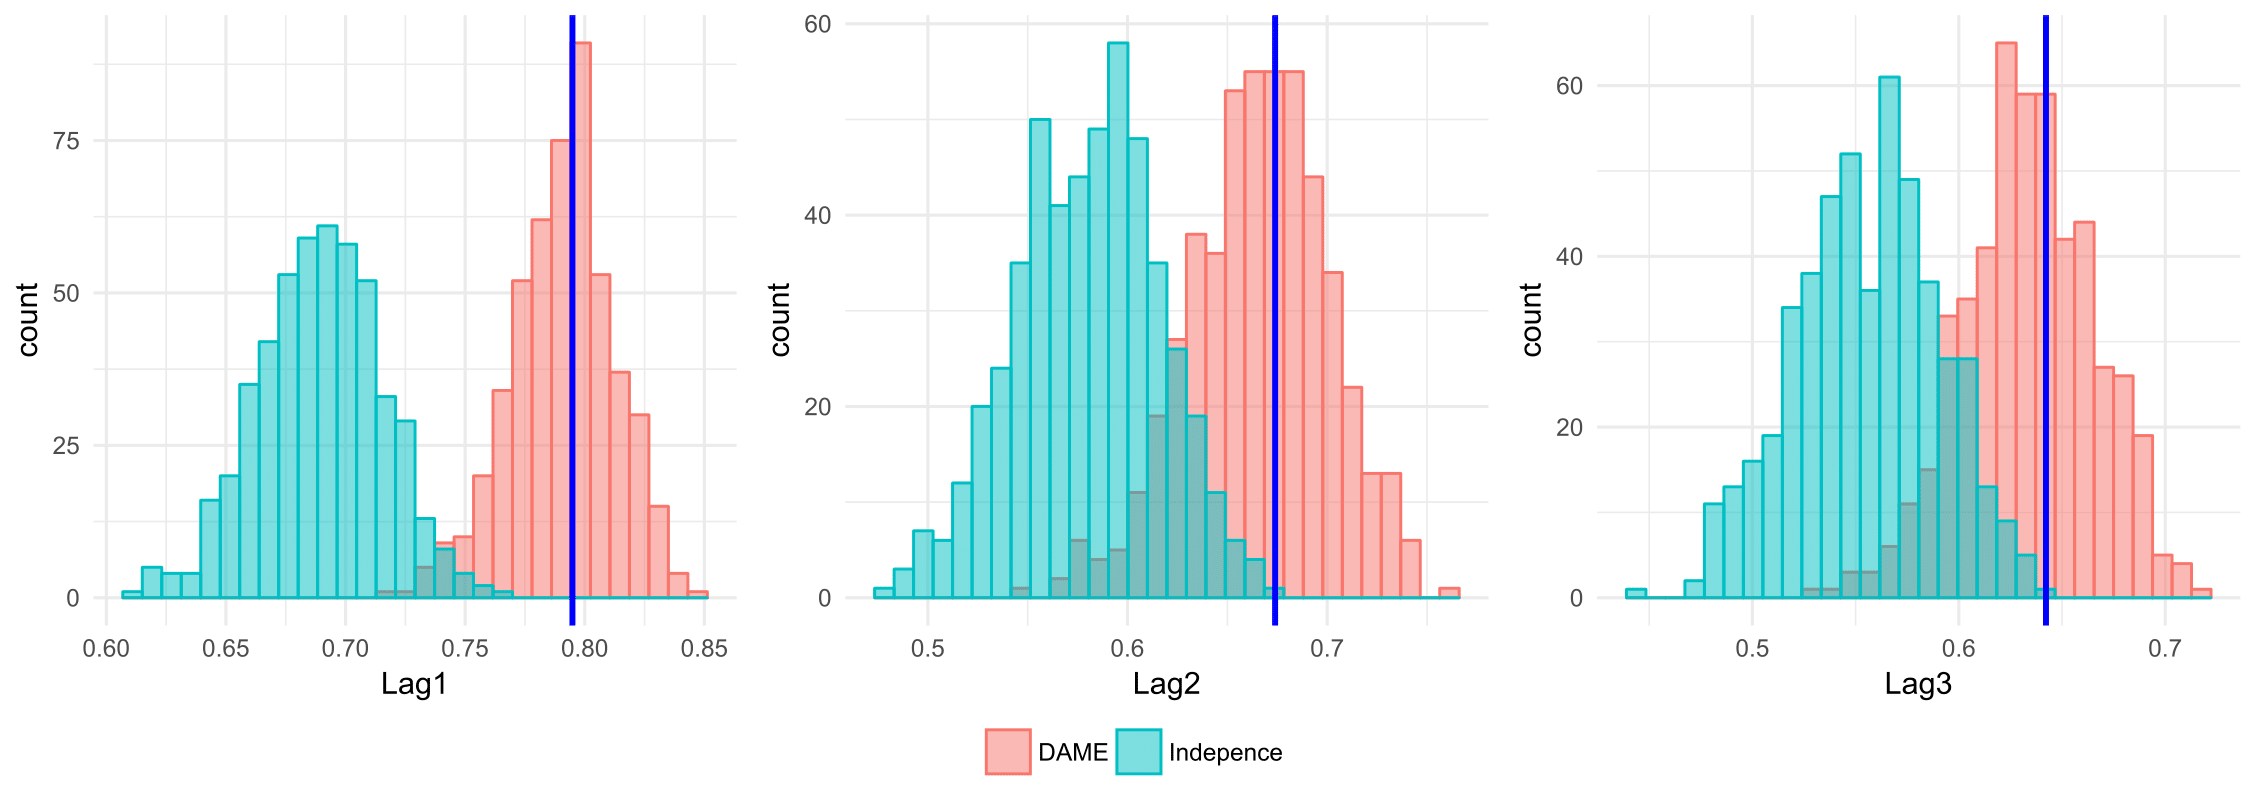
\includegraphics[width=1\textwidth]{plots_paper/correlations-1.png}	
	\caption {Histogram of posterior lagged degree correlations for $l=1,2,3$: the DAME model (\textit{red}) and independence model (\textit{green}), with the vertical lines representing observed $dc$ statistics.}
	\label{figure:correlationstudy}
\end{figure}
\subsection{Capturing Transitivity} \label{subsec: negative transitivity}
As introduced in Section \ref{sec: Introduction}, there exist two different types of transitivities, positive and negative transitivity, and the parameterization without $\mathbf{D}$ term (i.e. $\boldsymbol{u}'\boldsymbol{u}$) is not able to capture negative transitivity. We test if the DAME model can explain both positive negative transitivities by conducting another set of simulation study. Similar to Section \ref{subsec: correlation}, we generate $\mathbf{Y}$ with $N=20$, $T=10$, $P=1$, $R=2$, and $\forall (a, b) = (2, 1)$. Considering that our new goal is not to estimate temporal correlations but to represent transitivity effects, this time we fix $d^t_{r} = \pm 2$ for $r=1,\ldots, R$ and $t=1,\ldots,T$ such that the generated network exibits positive, mixed, or negative transitive features, respectively. Again, we run 6,000 MCMC iterations and discard the first 1,000 with thinning interval of 10. We fix the range parameter $\kappa$'s at their true values (i.e. $(\kappa^\beta, \kappa^\theta, \kappa^d) = (0, 0, 0)$) and do not estimate the covariance paramters (i.e. independence model) such that all paramters and the resulting dynamic network is independent across any timepoint, thus the difference in model performance only originates from the multiplicative effects formulations---$\boldsymbol{u}^\prime \mathbf{D}\boldsymbol{u}$ and $\boldsymbol{u}^\prime \boldsymbol{u}$. If we estimated $\kappa$'s for this comparison, the difference in results may not only arise from the formulation of multiplicative effects, but also possibly come from lack of correlation structure in $\boldsymbol{u}^\prime\boldsymbol{u}$ because our modeling framework do not embed any temporal correlation on the latent positions $\boldsymbol{u}$ in Section \ref{subsec: Model formulation}.   \\ \newline 
Figure \ref{figure:negativitystudy} illustrates a graphical comparison between the two formulations of the multiplicative random effects, with respect to the degree of the first, second, and third moments of the edge matrix (i.e. degree($\hat{\mathbf{Y}}$) degree($\hat{\mathbf{Y}}^2$) and degree($\hat{\mathbf{Y}}^3$), respectively). We a randomly choose a node and show its degree distribution over time. For the case of positive transitivity ($\forall d^t_{r} =+2$), our model and its alternative do not show significant differences; both formulations achieve great performance in replicating the degrees of the first, second, and third moments of the edge matrix. On the contrary, when we fit the network with mixed ($\forall d^t_{r=1} =-2$ and $\forall d^t_{r=2} =+2$) or negative transitivity ($\forall d^t_{r} =-2$), the two formulations reveal noticeable differences. While the DAME model can still recover the true degrees in first to third moments, the alternative model without $\mathbf{D}$ term shows inaccuracy in simulating a network that is close to the true data. Not only the alternative $\boldsymbol{u}^\prime \boldsymbol{u}$ model introduces bias, but also it yields significanlty wider interval estimates, implying lower precision compared to the DAME model. In addition, the evidence of $\boldsymbol{u}^\prime \boldsymbol{u}$ model's failure to capture the transitivity effects becomes larger as the network tends toward stronger negative transitivity and also as we move to the degree statistics in higher moments. These findings strongly support our choice of $\boldsymbol{u}^\prime \mathbf{D}\boldsymbol{u}$ formulation over $\boldsymbol{u}^\prime \boldsymbol{u}$ to model networks with various types of transitivity.
\begin{figure}[H]
	\centering
			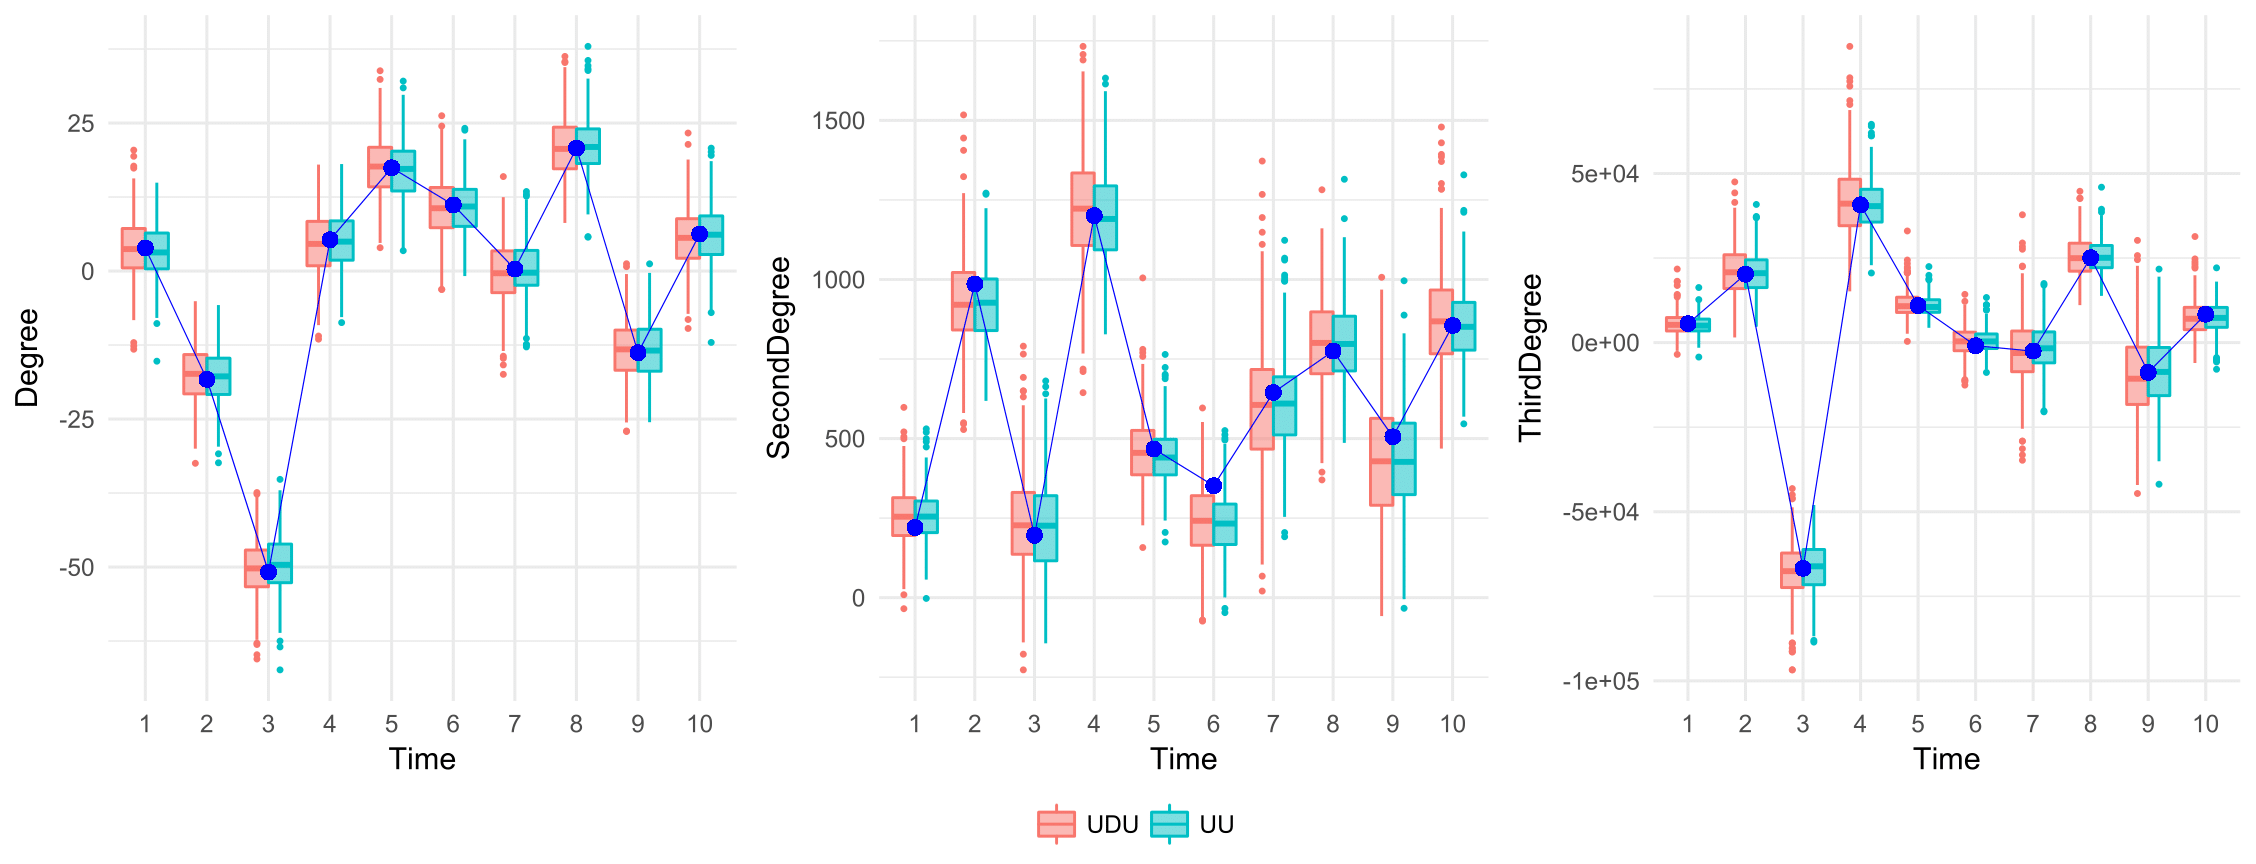
\includegraphics[width=0.895\textwidth]{plots_paper/newpositiveD-1.png}	
		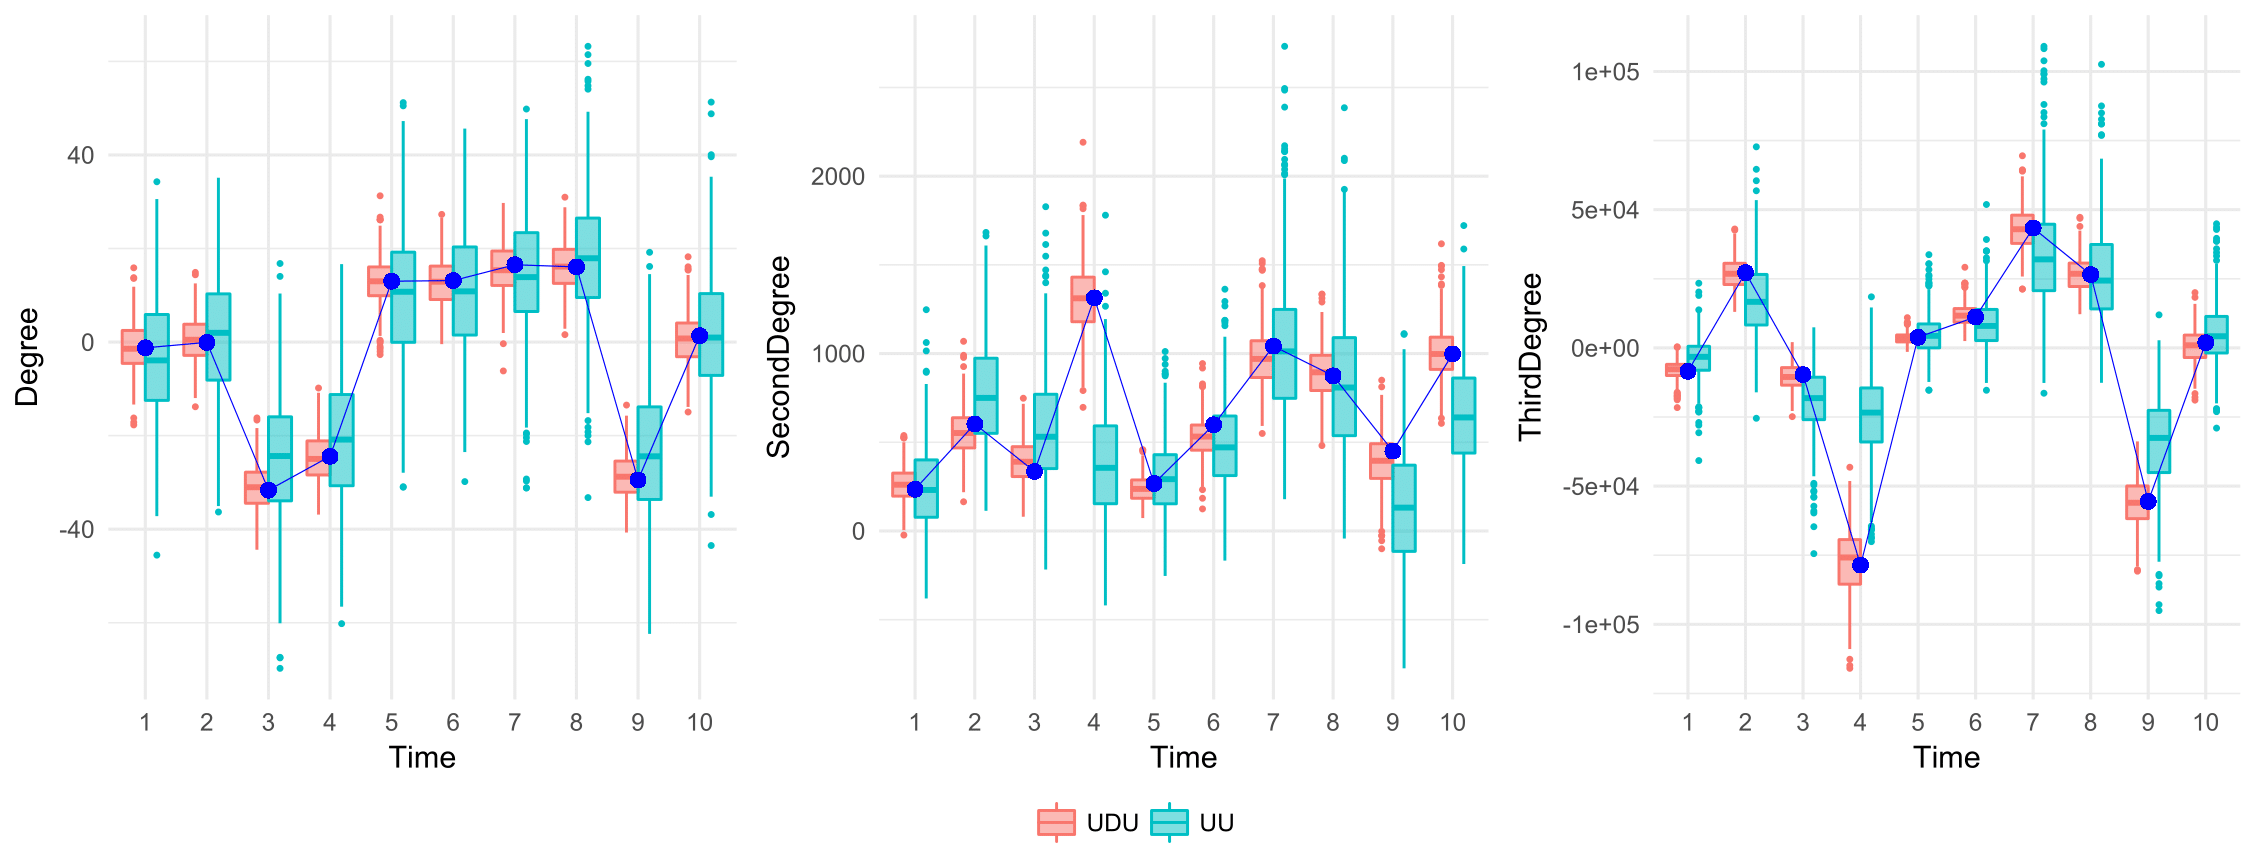
\includegraphics[width=0.895\textwidth]{plots_paper/newmixedD-1.png}	
						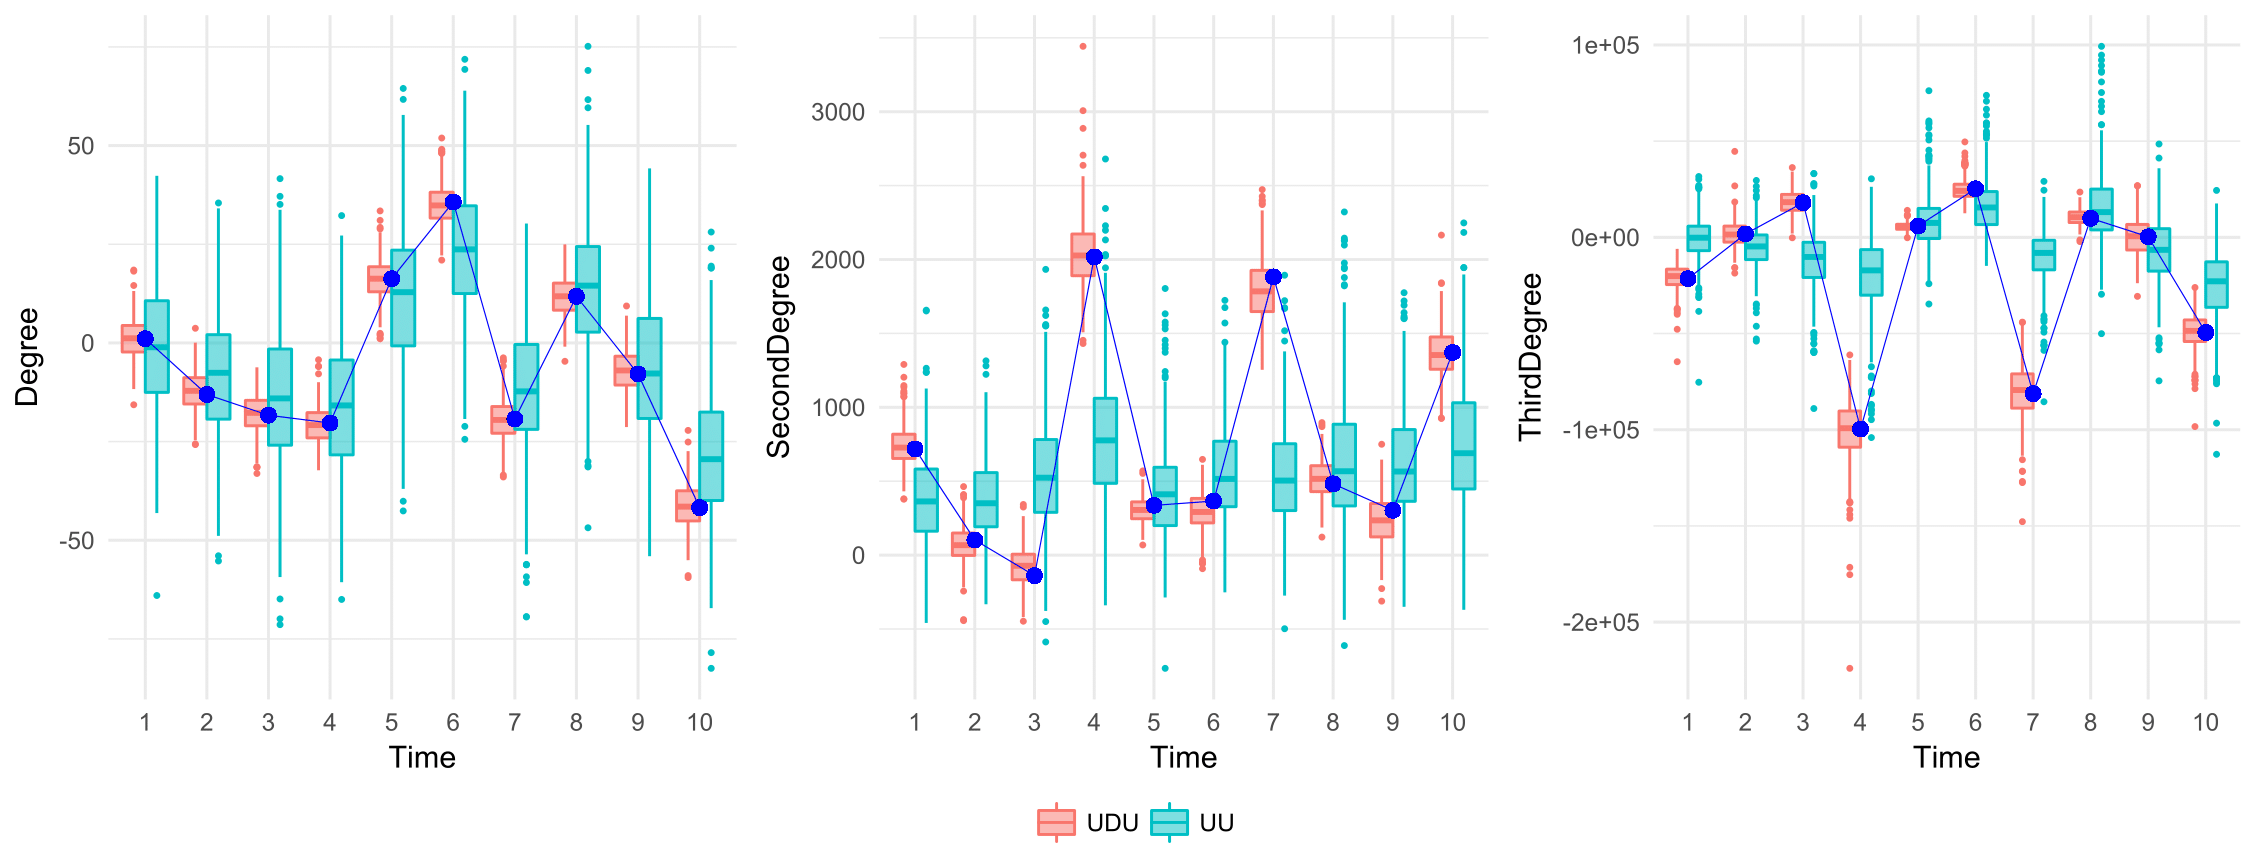
\includegraphics[width=0.895\textwidth]{plots_paper/newnegativeD-1.png}	
	\caption {Posterior distribution of the degree statistics in the first (\textit{left}), second (\textit{center}), and third (\textit{right}) moments corresponding to positive transitivity (\textit{upper}), mixed transitivity (\textit{middle}), and negative transitivity (\textit{lower}): the DAME (red) and $\boldsymbol{u}^\prime \boldsymbol{u}$ model (\textit{green}), with the dots representing observed statistics.}
	\label{figure:negativitystudy}
\end{figure}

\section{Analysis of the United Nations Voting Network}\label{sec: UNvoting}
\subsection{Data}\label{subsec: data processing}
Votes in the United Nations General Assembly (UNGA) have been analyzed in many political science papers \citep{voeten2000clashes,voeten2004resisting,bearce2007intergovernmental,mattes2015leadership,bailey2017estimating}, and became the standard data sources to measure the state preferences. The study of state preferences in international politics is one of the most important topics in the field of international relations \citep{wendt_1994}. With regard to policy implications, for instance, states are the key actors at the global stage, knowing their preferences towards each other and tastes on difference issues, helps us predict future foreign policies and state behaviors. Unfortunately, the existing studies ignore three important features of the dataset. First, votes are highly correlated across timepoints, because they are the reflections from history. \cite{bailey2017estimating} proposes a dynamic ordinal spatial IRT (item response theory) model and allows for better inter-temporal comparisons. However, their model again limits the temporal dependence to be lag 1 (i.e., Markovian assumption---votes at time $(t+1)$ is only dependent on votes at time $t$). Second, although the researchers have viewed ``voting" as dyadic behavior and thus used dyadic similarity indicators such as affinity or S scores \citep{gartzke1998kant,signorino1999tau}, to our knowledge, the United Nations voting data has never been analyzed using the network models. Third, third-order dependence (e.g., transitivity and clusterability) has not been investgated despite the fact that voting decisions are not limited to dyadic calculations---country A's decision to vote along the line with country B might well be influenced by a country C's decision. In order to overcome the limitations and provide the new insight at the same time, we apply the DAME model to the United Nations General Assembly roll-call votes, from 1983 to 2014.\\ \newline
Here are the data processing procedures used in the analysis. First, we determine the countries to be included in this analysis by 1) taking the intersection of countries available for each predictors (e.g., votes, polity score, GDP) and then 2) dropping countries with missings over 10 years, while the remaning missings are imputed using the data from previous years. Full list of countries and their abbreiviations are listed in Appendix \ref{appendix: countrylist}. Specifically, the voting data was obtained from \cite{12379_2016}, where we use the subset of the votes called `important votes', identified by U.S. State Department of Voting Practices in the United Nations as ``votes on issues which directly affected important United States interests and on which the United States lobbied extensively." \footnote{For example, in 2001, important votes include `Israeli Actions in the Occupied Territories', `Peaceful Settlement of the Question of Palestine', `U.S. Embargo Against Cuba', and `Nuclear Disarmament'. More can be found in \url{https://www.state.gov/p/io/rls/rpt/}}. The number of important votes on average is 12 per year, ranges from 6 to 28. We only use important votes from the original data because non-important votes show high agreement rate over the time period (1983--2014) with little variations, and thus may not strongly reflect state preference of the countries. Annual averge voting similarity index (i.e., agreement rate) of non-important votes are provided in Appendix \ref{appendix: unimportantstat}. We then construct the response $\mathbf{Y} = \{\mathbf{Y} ^1,\ldots,\mathbf{Y} ^{32}\}$, where each $\mathbf{Y} ^t$ is $97\times 97$ matrix of a voting similarity index (0--1) computed using 3 category vote data (Y = “yes” or approval for an issue; A = abstain; N = “no” or disapproval for an issue)\footnote{Voting similarity index between the two countries $i$ and $j$ at year $t$ is calculated as (Number of votes $i$ and $j$ agreed at year $t$) / (Number of votes $i$ and $j$ both participated at year $t$)}, which corresponds to the variable `agree3unimportant' in the original dataset. Note that abstention is counted as half-agreement with a yes or no vote \citep*{12379_2016}, while two abstention is treated as full-agreement. For basic summary of Unite Nations voting data for important votes, see Appendix \ref{appendix: summarystat}. \\ \newline
As an exploratory data analysis, Table \ref{table:corr} illustrates the lagged degree correlation $dc$ (defined in Equation \ref{eqn:dc}) of the observed dataset to measure how strong the Unite Nations voting data is correlated over time. There exists strong positive correlation in how the countries vote in the United Nations General Assembly over time, and as the distance between two timepoints become larger the correlation tends to be weaker. This provides solid evidence to support the use of a non-Markovian model, and therefore our model with Gaussian process specifications may be one of the appropriate appraoches to account for the strong temporal dependence in this dataset.\\
\begin{table}[ht]
	\centering
	\begin{tabular}{ |c|c|c|c|c|c|c|c|c|c|c|} 
		\hline
		{Lag}	& 1 & 2& 3& 4& 5& 6& 7&8&9&10 \\ \hline
		$dc$ & 0.732&0.623&0.513&0.435&0.395&0.315&0.263&0.158&0.164& 0.203\\\hline
	\end{tabular}
	\caption {Lagged degree correlation $dc$ of the United Nations Voting Data for $l=1,\ldots, 10$.}
	\label{table:corr}
\end{table}
\newline Next, to dynamically model the United Nations voting network in relation to other variables reflecting international relations, we combine $P=5$ different dyadic variables from the Correlates of War (COW) data \citep{gibler2008international}, Polity IV data \citep{marshall2014polity} and the International Monetary Fund (IMF)'s Direction of Trade Statistics (DOTS) and International Financial Statistics (IFS) data, and construct the observed edge covariates $\mathbf{X}$. For every $p=1,\ldots,P$, we set the explanatory variable $X^t_{ijp}$ as below.
\begin{itemize}
	\item [1.] $\mbox{Intercept}^t_{ij}$: constant 1,
	\item [2.] log($\mbox{distance})^t_{ij}$: log of the geographic distance between country $i$ and country $j$,
	\item [3.] $\mbox{Alliance}^t_{ij}$: 1 if country $i$ and country $j$ have alliance, and 0 otherwise,
	\item [4.] $\mbox{Polity difference}^t_{ij}$: absolute difference in polity IV number between country $i$ and country $j$,
	\item [5.] $\mbox{Lower trade-to-GDP ratio}^t_{ij}$: index of economic dependence using bilateral trade weighted by each country's gross domestic product (GDP), as defined in \cite{gartzke2000preferences} $$min\Big(\frac{\mbox{Trade}_{ijt}}{\mbox{GDP}_{it}}, \frac{\mbox{Trade}_{ijt}}{\mbox{GDP}_{jt}}\Big),$$
	\item [6.] $\mbox{Common language}^t_{ij}$: indicator of whether country $i$ and country $j$ share the same language,
\end{itemize}
where all covariates are symmetric (i.e., $X^t_{ijp}=X^t_{jip}$). Note that intercept is included to account for the baseline degree of agreement at each timepoint. Two variables---log($\mbox{distance}$) and common language---are time-invariant covariates, although their coefficients may vary over time. Correlations between the covariates are attached in Appendix \ref{appendix: correlations}.\\\newline
We specify the matrix of availability $\mathbf{A}$ introduced in Section \ref{subsec: varying number of nodes} to reflect some countries' non-participation in the United Nations Genearl Assembly (UNGA): 
\begin{itemize}
	\item[1.]  North Korea (PRK) have structural missings from $t = 1$ to $t = 8$:\\
	-- North Korea did not vote until North Korea and South Korea have simultaneously admitted to the United Nations in 1991.
	\item[2.] South Korea (ROK) have structural missings from $t = 1$ to $t = 8$:\\
	-- South Korea did not vote until North Korea and South Korea have simultaneously admitted to the United Nations in 1991.
	\item [3.] Russia (RUS) has structural missings from $t=1$ to $t =9$:\\
-- Russia succeeded the Soviet Union's seat, including its permanent membership on the Security Council in the United Nations after the dissolution of the Soviet Union in 1991. 
	\item [4.] Iraq (IRQ) has structural missings from $t =13$ to $t = 21$:\\
	-- The country did not participate the UNGA roll-call votes during 1995--2003. Under the rule of Saddam, Iraq was under severe sanctions from the international community including the United Nations since 1990.
\end{itemize}
Therefore, any missing values corresponding the country's missing period are treated as structural missings. As in Section \ref{subsec: varying number of nodes}, other random missing values are treated as random missing (and thus imputed). 
\subsection{Reduced-Rank Structure of Voting Network}\label{subsec: reduced rank}
In this section, we demonstrate the special low-rank structure of the voting network, which can be generalized into any other similarly constructed ``agreement" networks. For simplicity, we assume static network by fixing $T = 1$ and consider the $N \times N$ adjacency matrix $\mathbf{V}^1$ representing the network consists of a single vote. Since each entry of $\mathbf{V}^1$ denotes a voting similarity index (0--1) computed using 3 categories (“yes”, ``abstain", and “no”), the $(i, j)^{th}$ element $V^1_{ij}$ can only have three possible values:
\begin{equation*}
V^1_{ij} =\begin{cases}
1, & \mbox{agreement}\\
0.5, &\mbox{half-agreement (one abstain)}\\
0, & \mbox{disagreement}\\
\end{cases}
\end{equation*}
which implies perfectly-transitive property of the agreement network---i.e. if there is an agreement between $i$ and $j$, and also between $j$ and $h$, then there must be an agreement between $i$ to $h$. Therefore, any two edges sharing one node, such as $V^1_{ij}$ and $V^1_{jh}$, automatically determines the third edge between the unshared nodes $V^1_{ih}$. This constraint makes the maximum rank of $\mathbf{V}^1$ to be 3. In other words, if we were to apply the DAME model to this type of single vote network (without any additive effects and explanatory variables), the maximum rank of dimension for the multiplicative effects we could fit for low rank factorization is $R=3$. Moreover, each dimension $r$ in the estimated $\boldsymbol{u}$ and $\mathbf{D}$ can be viewed as the distinct constructs behind the vote. \\ \newline
Although it is definitely worth understanding the constraint behind single votes, this is not a practical issue in modeling the United Nations voting network, where we aggregate multiple votes per year (minimum number of important votes per year is 6). When we add $M$ number of matrices representing each vote, the aggregated matrix $\mathbf{V} = \mathbf{V}^1+\mathbf{V}^2+...+\mathbf{V}^M$ gets closer to the full rank thus we no longer need to concern about the maximum dimension of the multiplicative effects in fitting the DAME model. Furthermore, including the observed covariates $\mathbf{X}$ and additive random effects $\boldsymbol{\theta}$'s also relax the reduced rank structure, since the multiplicative effect $\boldsymbol{u}^\prime \mathbf{D}\boldsymbol{u}$ is modeled after we subtract those effects from the response (See Section \ref{sec: DAME}). Accounting for large variability in the observed covariates and additive random effects, the residuals no longer maintain the perfect transivity structure.
\subsection{Model Validation}\label{subsec: Model Validation}
We perform a model validation to check if the DAME model is an accurate and credible model for the data, and understand the role of different effects at the same time. We fit the model in Section \ref{subsec: Model formulation} with four different specifications: 1) with additive and multiplicative effects (DAME), 2) one with only multiplicative effects (ME), 3) one with only additive effects (AE), and 4) the last without any random effects (NO), where all four cases commonly include the 6 edge covariates in Section \ref{subsec: data processing}. Figure \ref{figure:modelvalidation} illustrates the comparison of posterior 95\% credible intervals of the degree statistics constructed from the model-simulated response $\hat{\mathbf{Y}}$. Out of 97 countries in total, we only present the results on the country ``Israel" (ISR) which reveals clear differences between the four models. First of all, we see huge benefit of correcting the bias when we add additive effects (AE), compared to the model with no random effects (NO). Next, when we compare between only additive effect (AE) and only multiplicative effect (ME), it is noticeable that the multiplicative effect model show significantly narrower width of credible intervals. This occurs since the additive effects have very small variance estimates while the multiplicative effects have larger variance estimates, which significantly lowers the error variance estimates $\hat\sigma_e^2$---which plays a big role in the precision of simulated data. Lastly, our model with both additive and multiplicative effects (DAME) outperforms the ME model in terms of both accuracy and precision. To be specific, the DAME model corrects the bias in the ME model by incorporating node-specific additive effects. Overall, not only the DAME model provides the most accurate estimates over time, but it also yields the narrowest 95\% credible intervals among the four. These findings emphasize the importance of including both the additive and multiplicative terms which enable the model to capture some features not explicable by fixed effects or only one random effect. More results and interpretation using the full DAME model are demonstrated in Section \ref{subsec: UNresult}, and the posterior predictive plots checking the overall degree distributions---aggregation of all nodes and timepoints---are provided in Appendix \ref{appendix: PPC}.
 \begin{figure}[ht]
 	\begin{center}
 		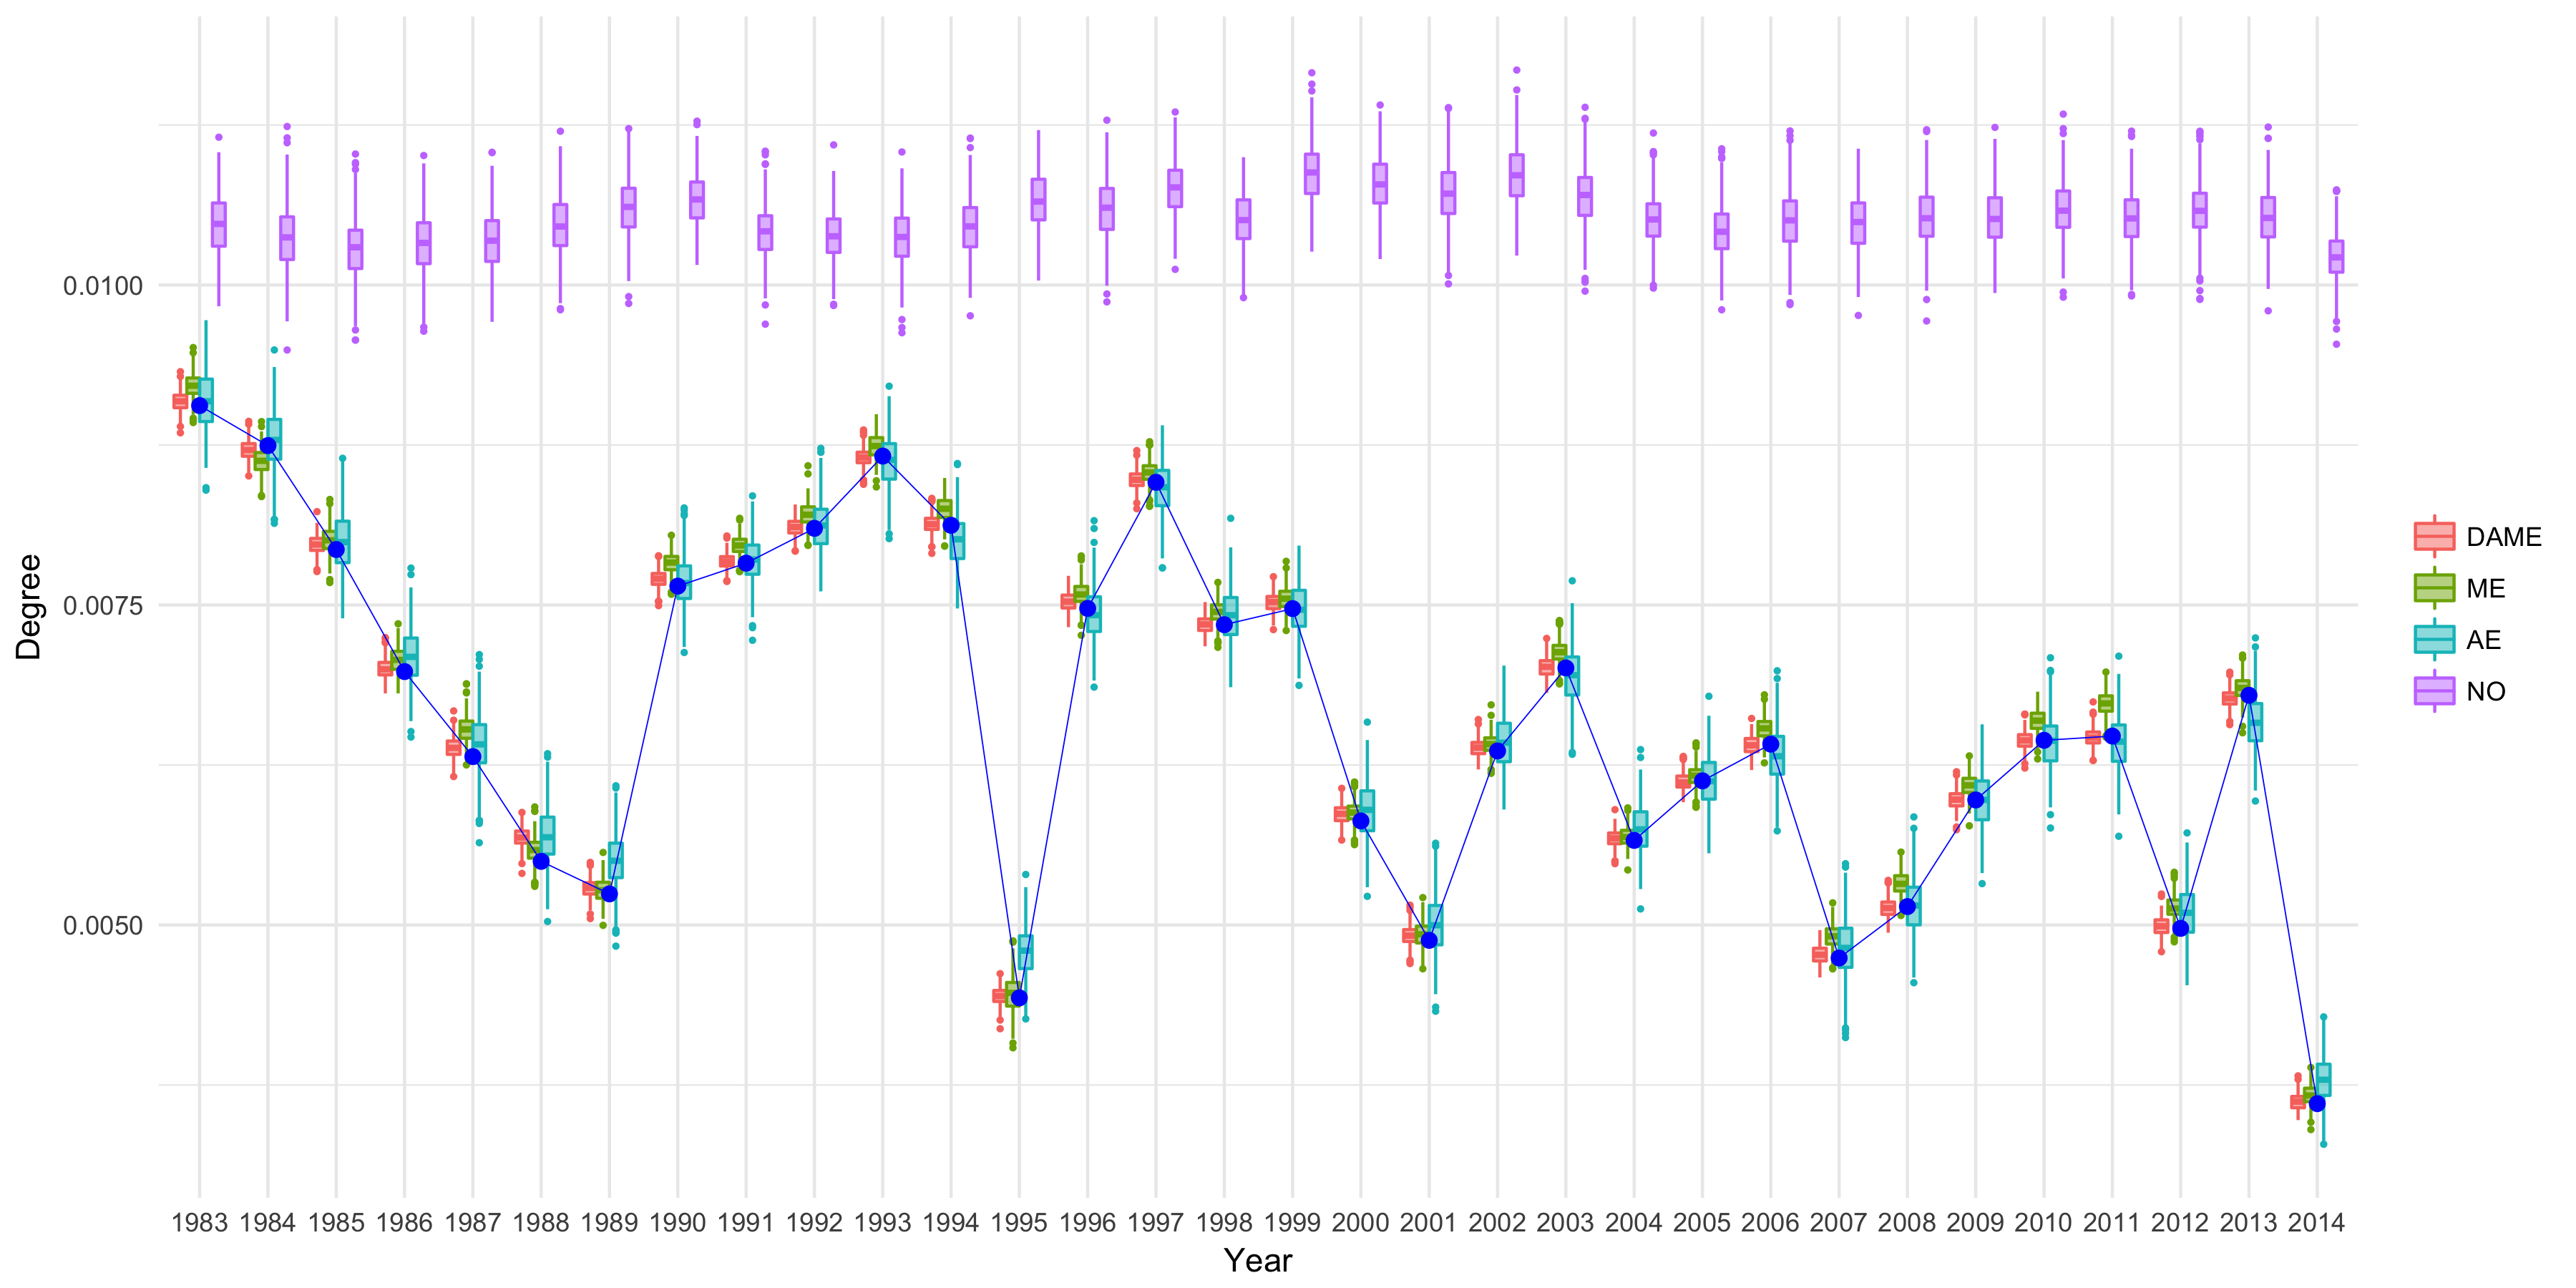
\includegraphics[width=1\textwidth]{plots_paper/ISR79.png}	
 	\end{center}
 	\caption {95\% credible intervals for posterior degree of Israel (ISR), comparing four models: the DAME (\textit{red}), only multiplicative effects (\textit{green}), only additive effects (\textit{blue}), and no random effects (\textit{purple}), with the dots representing the country's observed degree statistics.}
 	\label{figure:modelvalidation}
 \end{figure}
\subsection{Parameter Estimation and Interpretation}\label{subsec: UNresult}
Finally, we apply the DAME model to the United Nations General Assembly voting data which results in $N=97, T = 32$, and $P =6$. We choose the dimension of multiplicative effects as $R=2$ based on some preliminary experiments, where increasing the dimension do not significantly improve the model fitting (e.g., the estimated eigenvalue $d^t_{3}\approx 0$ for every $t=1,\ldots,T$). In this section, we present the results based on $30,000$ Gibbs iterations with a burn-in of $5,000$, where every $50^{th}$ sample was taken as a thinning. All model parameters including the GP parameters $(\kappa, \tau)$ are estimated according to Section \ref{subsec: posterior computation}, using the hyperparameters $(a, b) = (2, 1)$ and $\gamma = 5$. \\ \newline
Figure \ref{figure:interceptplot} shows the posterior mean estimates of the fixed effect coefficients $\{\boldsymbol{\beta}_p\}_{p=1}^P$ with their corresponding 95\% credible intervals. Overall, the effects of the covariates on the United Nations voting behavior change substantially over time, especially in the cases of geographic distance (i.e., log-distance) and economic effects (i.e., lower trade-to-GDP ratio). Most importantly, the ``critical junction" for these temporal changes seem to be around the end of Cold War, that is, late 1980s and early 1990s. For instance, the middle panel of the top row shows that during the Cold War period, the effect of distance on the United Nations voting behavior is overall negative (i.e., longer distance less similar votes), but much less significant than after early 1990s. It is likely that the votes in the United Nations were much more influenced by the overall ideological conflicts between the Soviet Union plus its satellites and the Western camp so the effect of geographical distance was weakened during the Cold War. Moreover, regarding the effect of polity---or distance in polity as we operationalize this variable---the result suggests that in general the political regime similarity does not often result in higher agreement in the United Nations General Assembly, at least for a few time periods included in the study, e.g., 1990--1995, 1997--2002, and 2005--2010. Scholars in the liberal tradition of international relations have long been arguing for shared norms, values and preferences between democracies; what the result here suggests that such similarity in preferences seem to be not sufficiently strong enough to sway countries' votes in the United Nations General Assembly, at least in the case of important votes.\\
\begin{figure}[ht]
	\begin{center}
		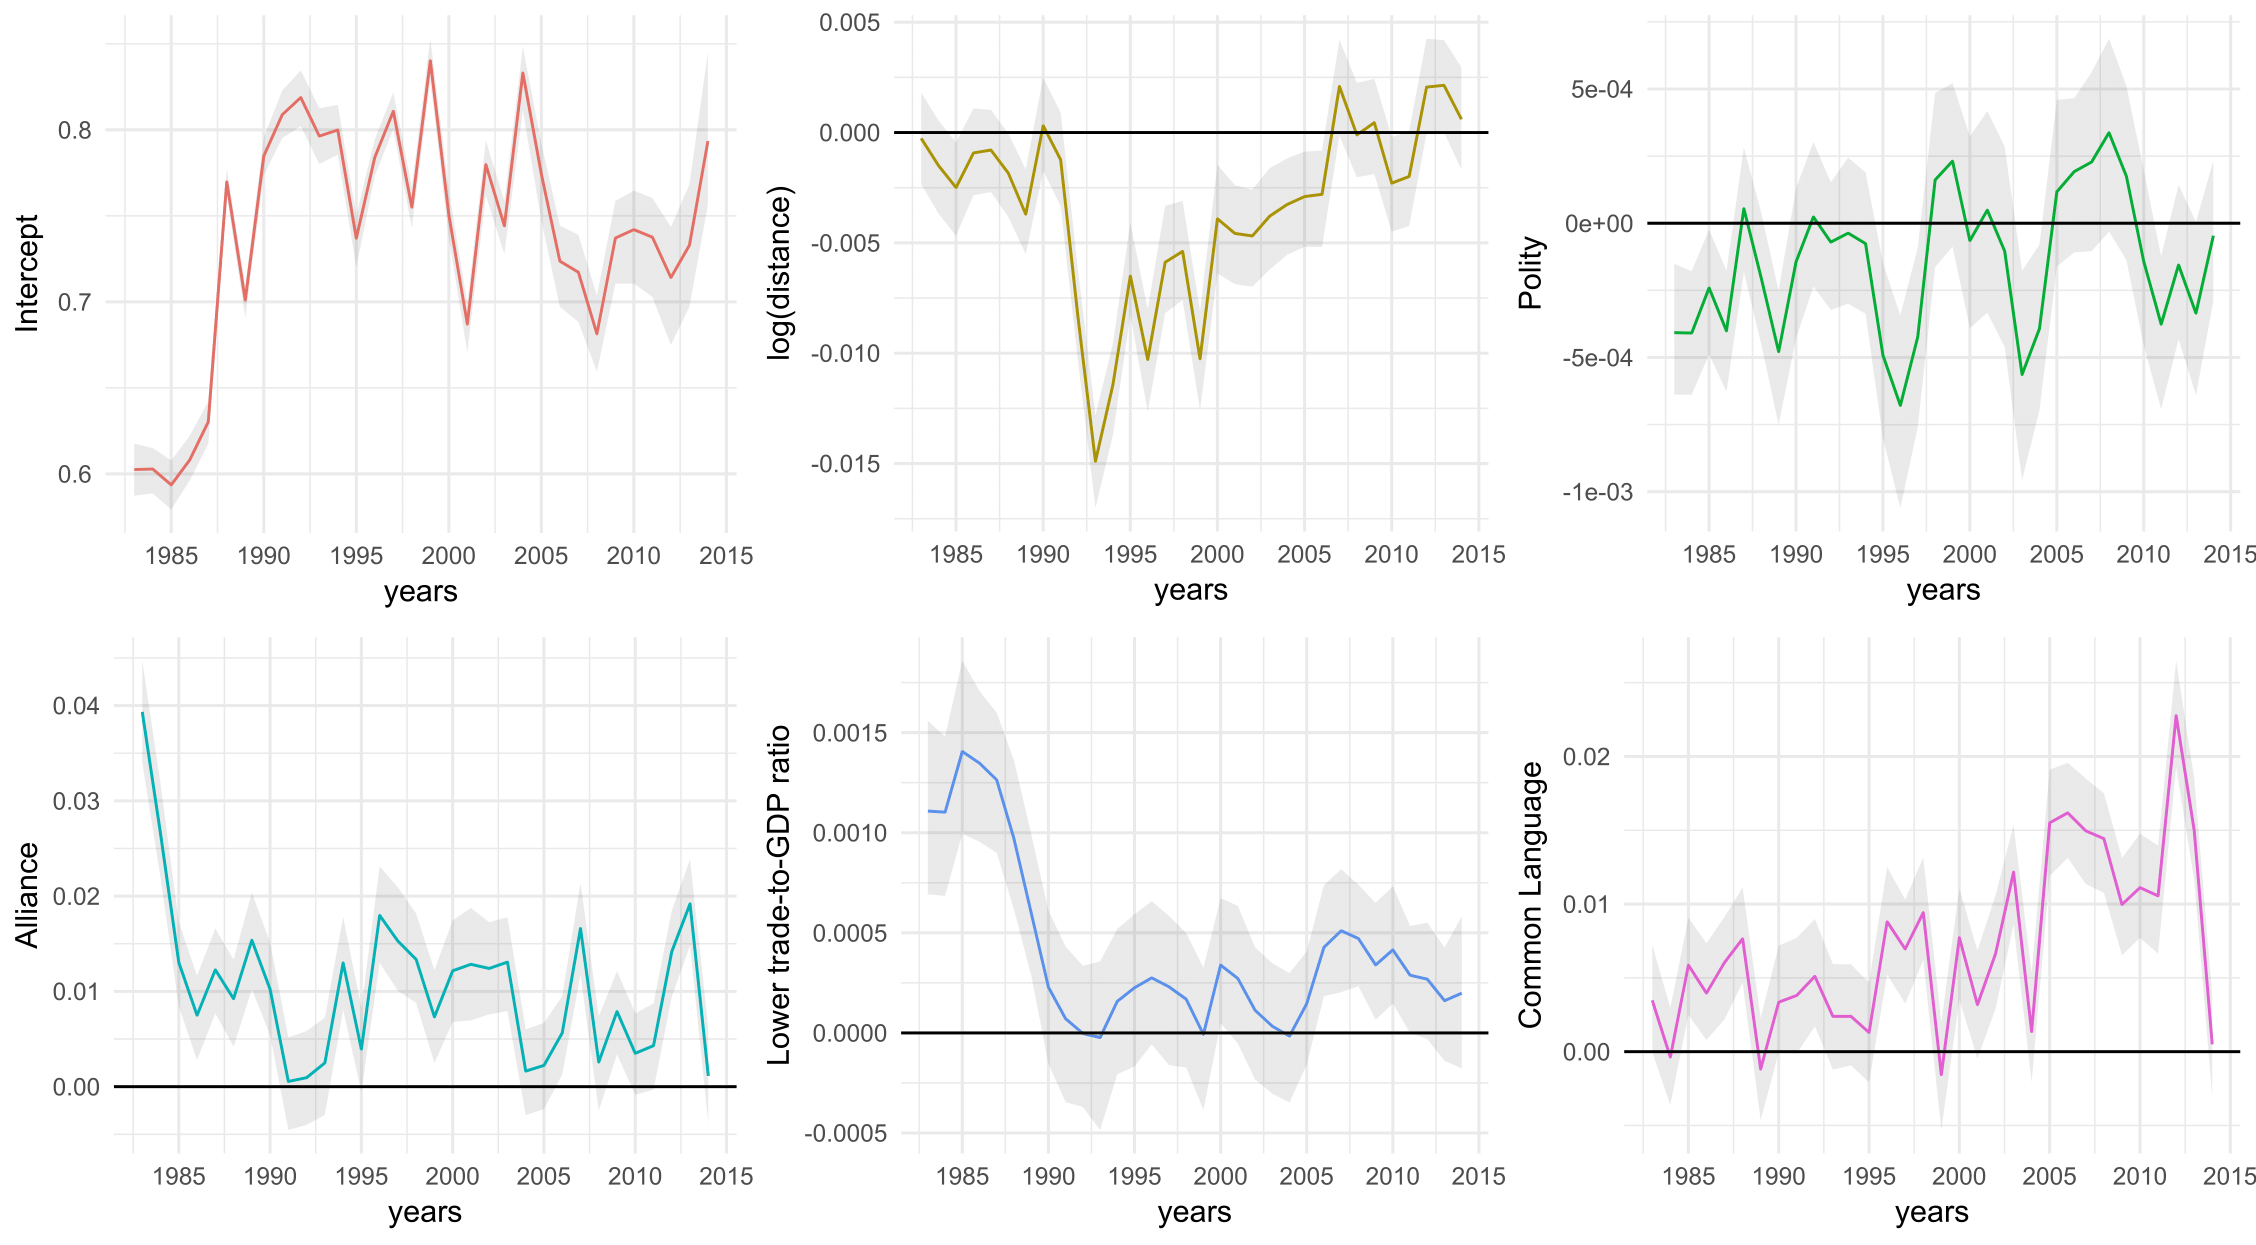
\includegraphics[width=1\textwidth]{plots_paper/betaplot-1.png}
	\end{center}
	 	\caption {Posterior mean estimates for the fixed effect coefficients $\boldsymbol{\beta}$ (\textit{colored line}): Intercept, log(distance), Alliance, Polity difference, Lower trade-to-GDP ratio, and Common Language, and their corresponding 95\% credible intervals (\textit{grey areas}). }
	\label{figure:interceptplot}
\end{figure}
 \begin{figure}[ht]
 	\begin{center}
 		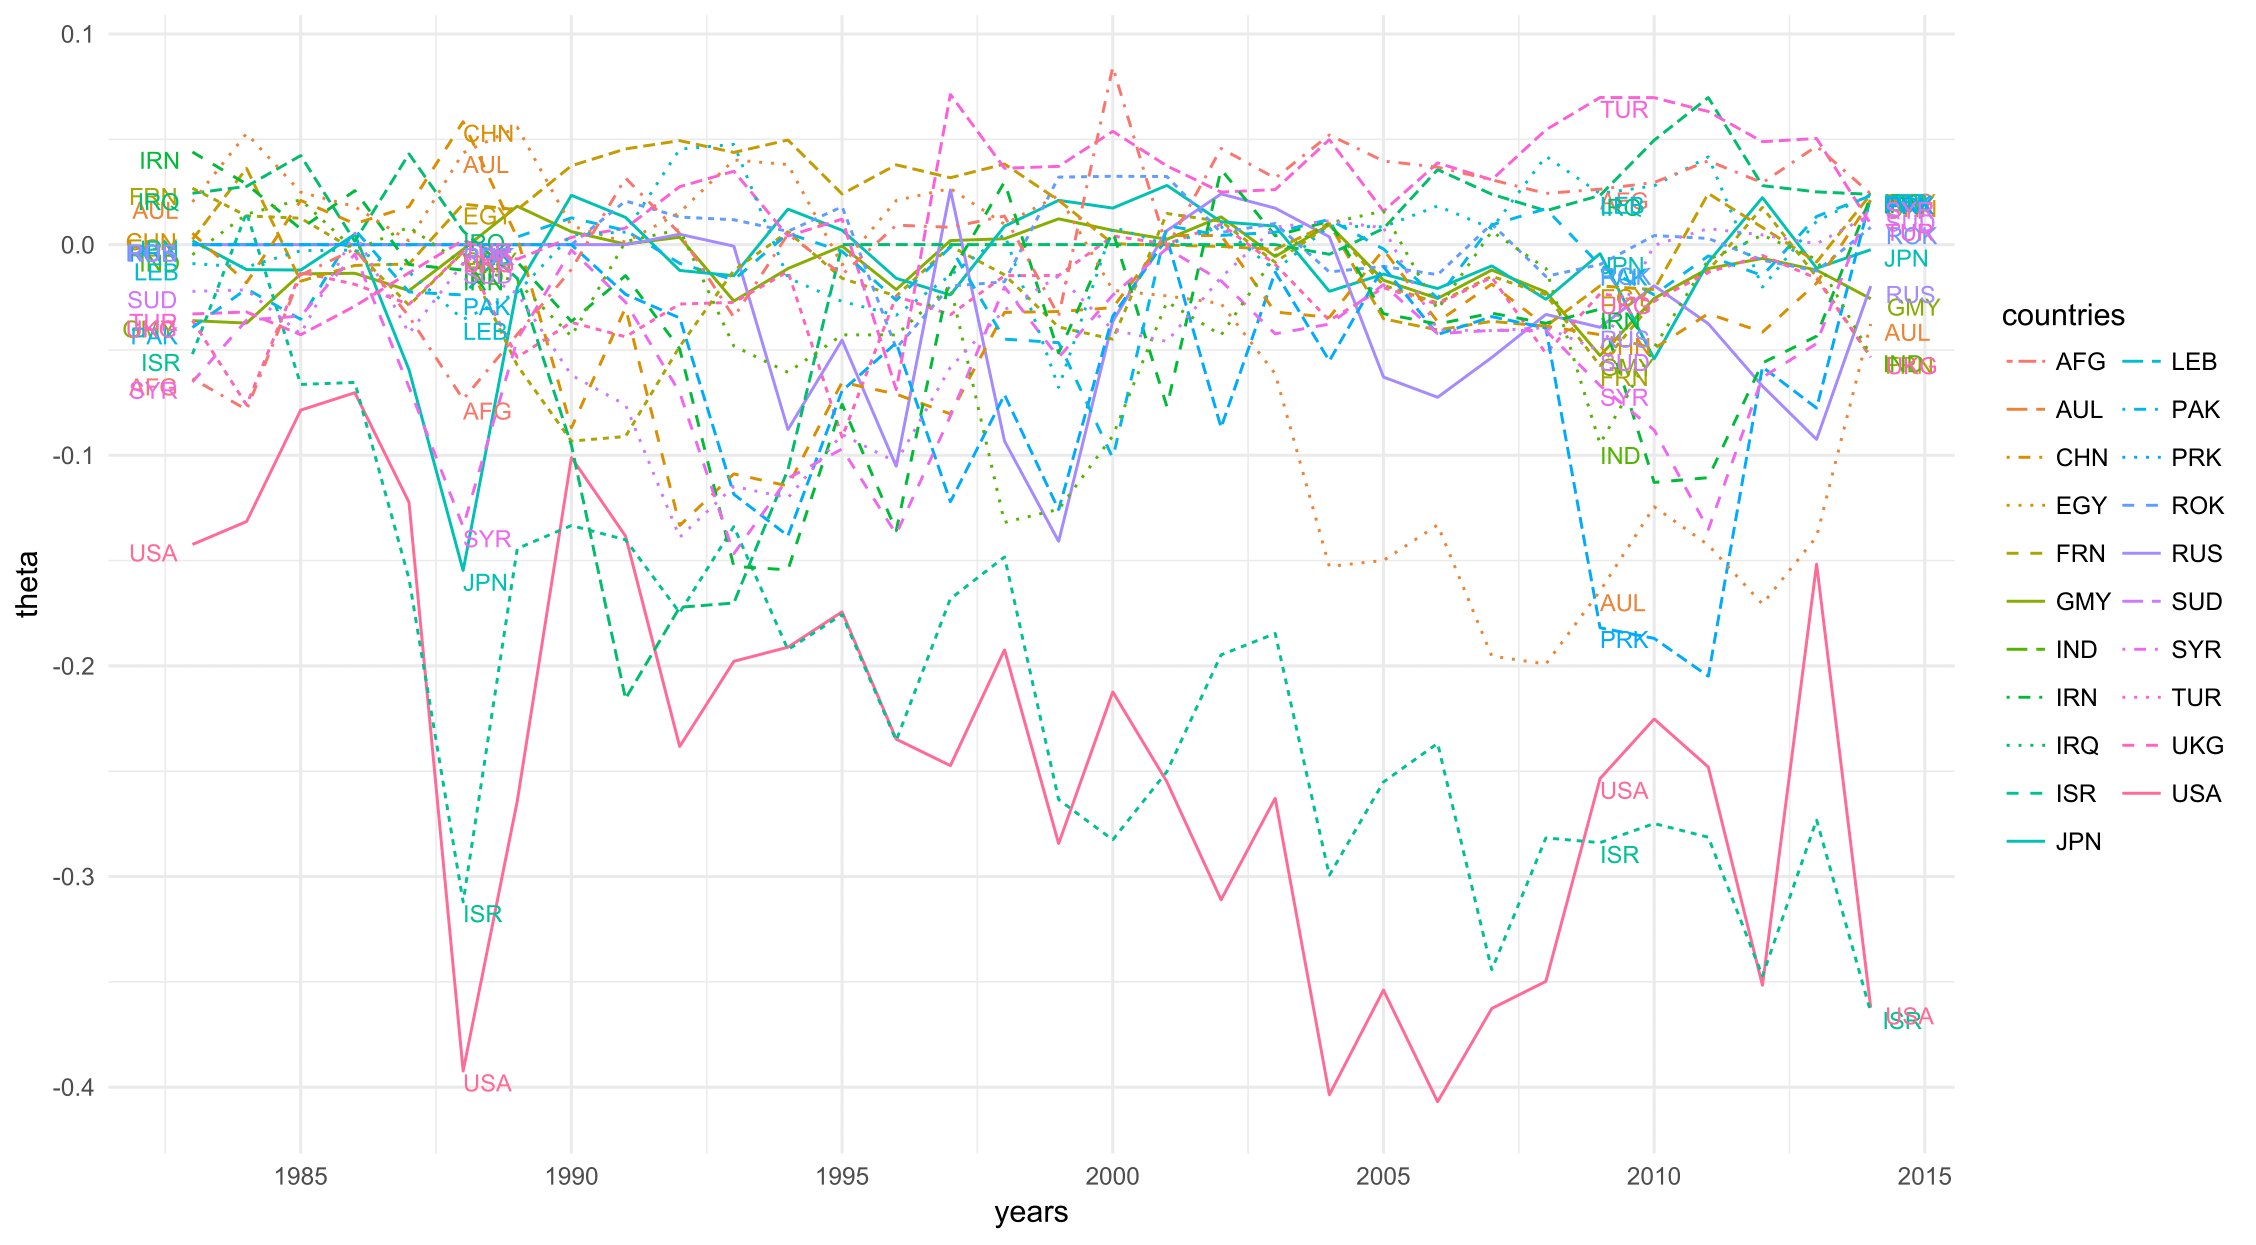
\includegraphics[width=1\textwidth]{plots_paper/thetaplot-1.png}	
 	\end{center}
 	\caption {Posterior mean estimates for the additive random effect estimates $\theta$.}
 	\label{figure:thetaplot}
 \end{figure}
 \newline\noindent After controlling for the observed covariates, we move on to the analysis of random effects, both additive and multiplicative ones. For clear visualization, we only present the result from 21 countries, where the countries are chosen based on the most active countries during the ten year period of 2004 -- 2014 \citep{hoff2015multilinear}. Here, the action types include negative material actions, positive material actions, negative verbal actions and positive verbal actions. The 21 most active countries are marked with $*$ in Appendix \ref{appendix: countrylist}. Figure \ref{figure:thetaplot} is the posterior mean estimates of each country's additive random effects or node-specific time-varying intercepts. Here, the United States (USA) and Israel (ISR) stand out with large negative additive random effects, suggesting that the two countries are less likely to cast the same votes with the rest of countries. Considering that the majority of votes are ``yes", we can infer that the two countries are more likely to vote for ``no" in general.\\ \newline
Finally, we provide the estimated latent positions of the 21 countries. To determine the posterior distribution of $\boldsymbol{u}$ without identifiability issue, we take eigendecomposition on every posterior sample of the multiplicative effect matrix $\boldsymbol{u}^\prime \mathbf{D}\boldsymbol{u}$, and let $\mathbf{D}$ be the diagonal matrix of $R$-number of eigenvalues and $\boldsymbol{u}$ be the corresponding eigenvectors. We then apply Procrustes transformation on each posterior estimate of $\boldsymbol{u}$ and multplied $\sqrt{\mathbf{D}}$, and obtain the posterior mean estimates and 95\% credible regions of $\boldsymbol{u}_i\sqrt{\mathbf{D}}$, for all $i=1,\ldots, N$. In Figure \ref{figure:UDplot}, the 21 countries are clearly not randomly distributed in 2-dimensional latent space as we see clear patterns of clustering of the countries. For example, in 1986, we observe a clear cluster including the USA and its Cold War allies---Japan (JPN), France (FRN), Germany (GMY), United Kingdom (UKG), Australia (AUL) and Israel (ISR). Moreover, it is interesting that Israel (ISR) is always close to the United States (USR) in the latent space. Specifically, in 2014, USA and Israel seem to have drifted away from other countries including the USA's traditional allies in Europe and Asia, which indicates that the two countries' alliance is beyond those observed variables such as economic factors.
\begin{figure}[ht]
  	\begin{center}  
  		 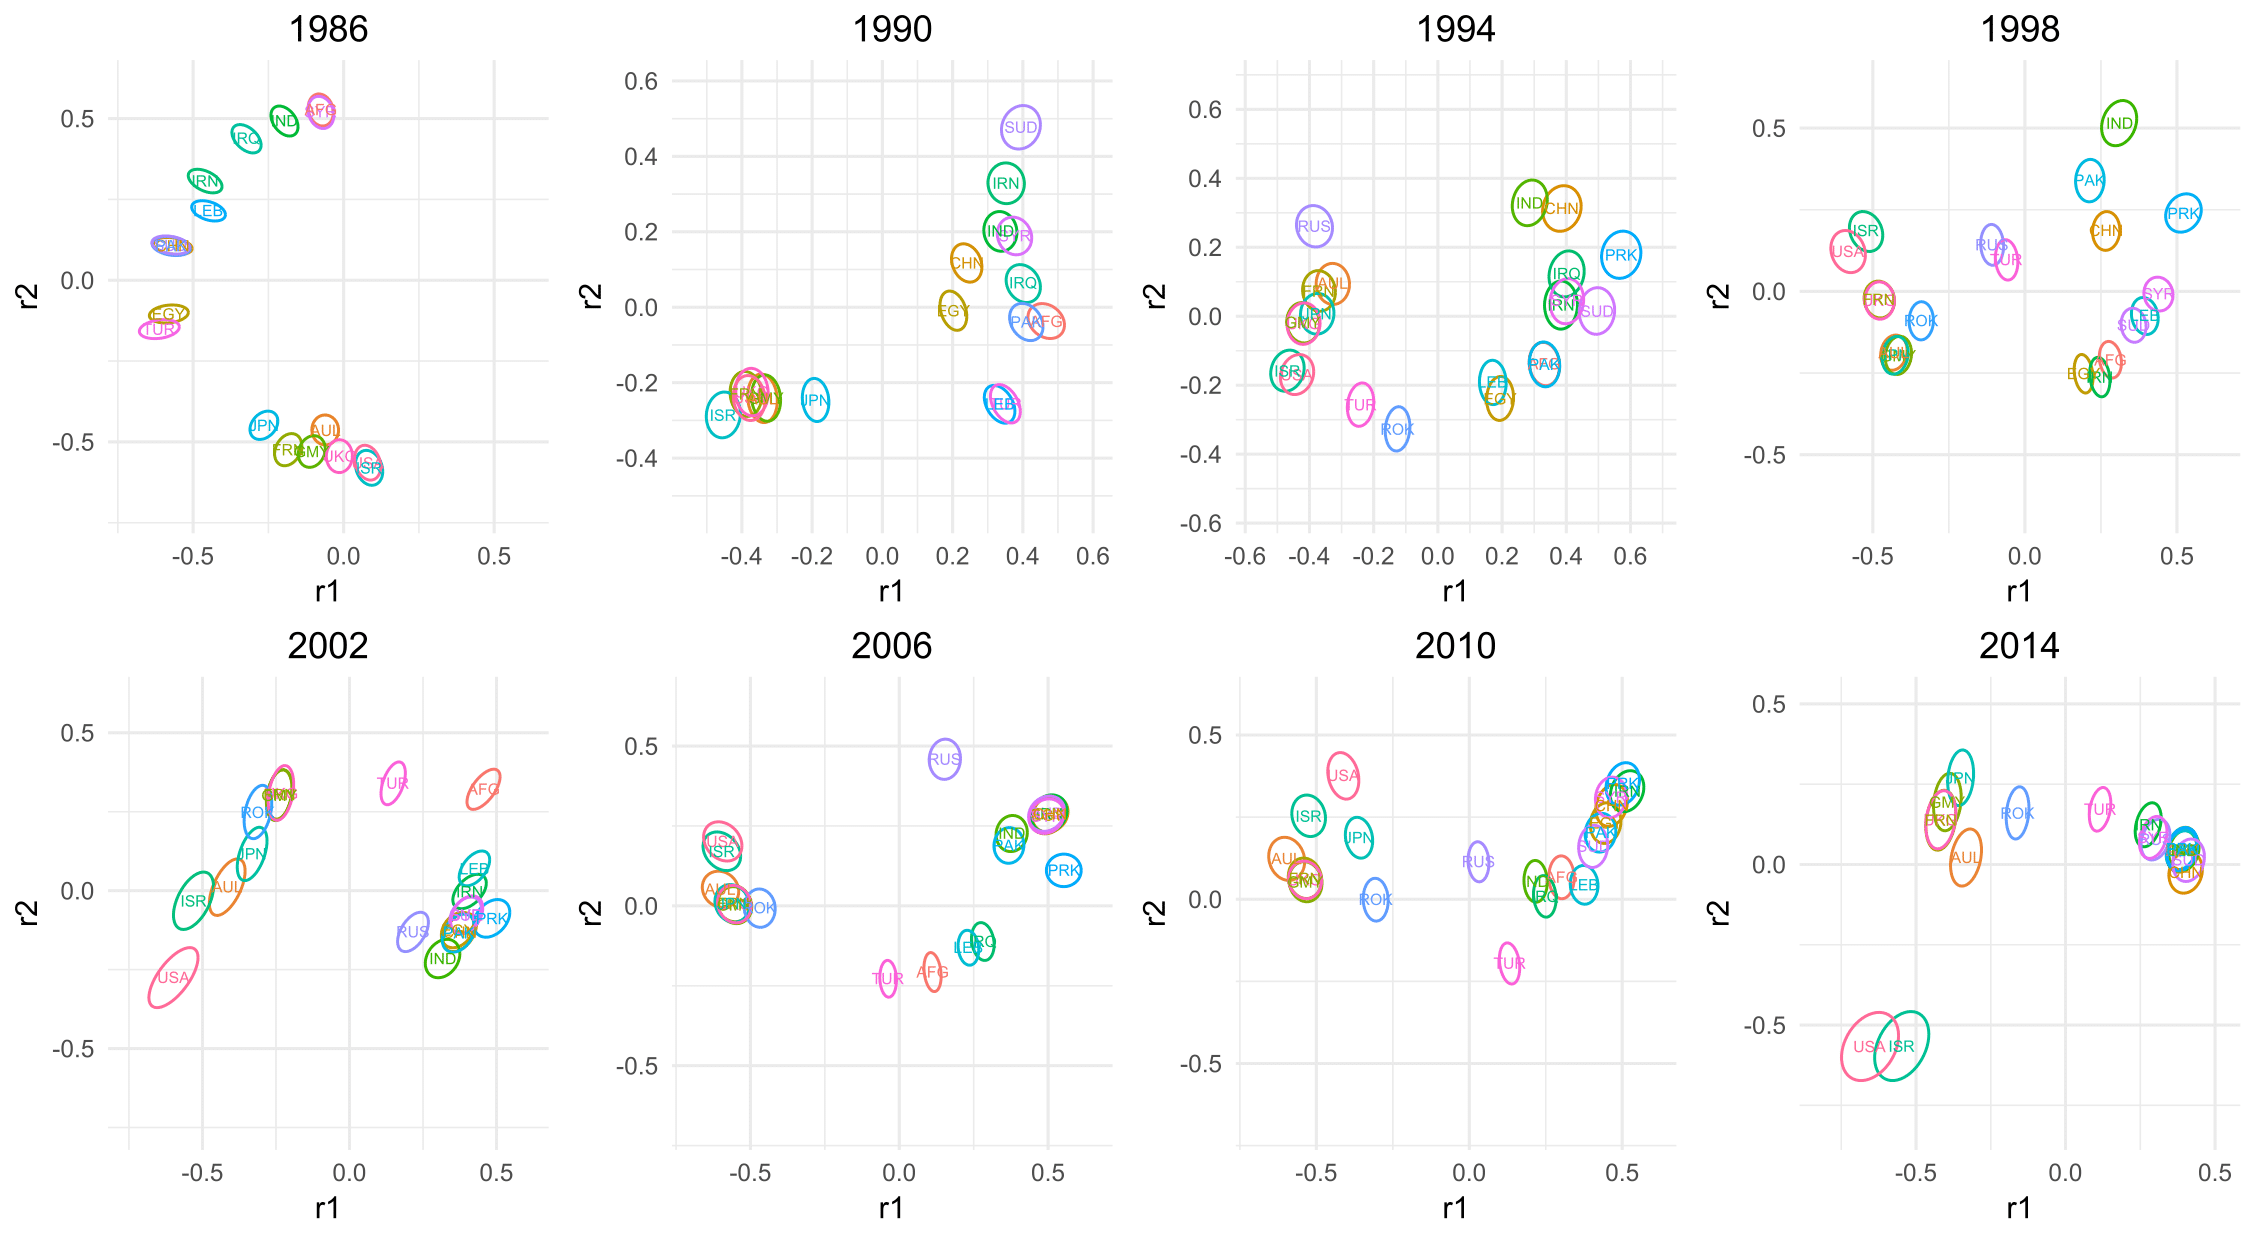
\includegraphics[width=1\textwidth]{plots_paper/UDU_reduced_8years-1.png}
  	\end{center}
  	\caption {Posterior mean estimates (\textit{texts}) for the multiplicative random effects and their corresponding 95\% credible regions (\textit{ellipses}) for the 21 selected countries for every 4 years between 1983 and 2014.  }
  	\label{figure:UDplot}
  \end{figure}
\section{Discussion}
As an extension of the additive and multiplicative effects (AME) model, the dynamic additive and multiplicative nework effects (DAME) model can flexibly learn the underlying time-varying strucutre in dynamic networks, while inferring the effects of node-specific and dyad-specific latent variables. Accounting the correlation structure of the networks makes better use of dynamic networks than modeling them as separate network snapshots. Our algorithm eliminates the need to make an arbitrary user-defined covariance structure, making it easier to understand the temporal dependence from the data itself. Information on temporal correlation is highly informative and thus leads to more accurate and precise inference. Further, the visualization of the model estimated time-varying parameters provides an effective temporal trend analysis of dynamic networks, as well as the descriptive visualization of higher-order dependencies over time.
\\\newline
We have demonstrated such effectiveness of our model by modeling the United Nations Voting networks. The model estimated additive and multiplicative effects and their changes over time reveal that the United Nations voting behavior reflects interesting and meaningful foreign policy positions and alliance of various countries, even after controlling for other edge covariates that are considered critical in the international relation studies. Although we illustrated the entire framework in the context of symmetric or undirected networks, our model can be easily extended to allow directed networks, following the additive and multiplicative effects model for the directed network \citep{minhas2016inferential}. Furthermore, the approach can be applied to binary and ordinal network data with appropriate link functions, while we currently only provide the application to continuous-valued networks. Finally, considering the recent explosion of network dataset with large number of timepoints, our model has a broad range of applicability, suggesting promising approach that can accommodate huge networks that span long period of time.
\newpage
\bibliographystyle{apalike}
\bibliography{BominBib2}
\newpage
\begin{appendices}
\section{List of Countries in Voting Network}\label{appendix: countrylist}
\begin{table}[H]
	\centering
\begin{tabular}{c|c||c|c}
	\hline
	Abbreviation&Country or area name &	Abbreviation&Country or area name\\
	\hline
			AFG* & Afghanistan & 	KUW & Kuwait\\
				ALB & Albania & LEB* & Lebanon\\
			ALG & Algeria & LIB &Libya \\
		ANG & Angola 	& MAA&  Mauritania\\
		ARG& Argentina	&MEX &Mexico \\
		AUL* & Australia&MLI&Mali\\
		BAH & Bahrain	&MOR & Morocco\\
	BEN & Benin 	&MZM & Mozambique\\
			BFO & Burkina Faso 	&NEW & New Zealand \\
	BNG&  Bangladesh	& NIC& Nicaragua\\
			BOL& Bolivia	& NIG &      Nigeria\\
		BRA &Brazil&NIR & Niger\\
				BUI & Burundi &NOR &Norway \\
		BUL & Bulgaria	&NTH &  Netherlands\\
		CAN & Canada	& OMA & Oman\\
		CAO & Cameroon	&PAK* & Pakistan\\
		CEN & Central African Republic	&PAN & Panama\\
			CHL & Chile &PAR & Paraguay\\
			CHN* & China	& PER & Peru \\
		COL & Colombia	&PHI & Philippines\\
			CON & Congo		&POL & Poland\\
			COS & Costa Rica&POR & Portugal\\
			DEN& Denmark	 & PRK* & North Korea\\
			DOM & Dominican Republic	&QAT & Qatar\\
		ECU &Ecuador 	&ROK* & South Korea\\
			EGY* & Egypt	&RUS* & Russia\\
				FIN & Finland	&RWA & Rwanda\\
			FRN* & France&SAL & El Salvador\\
			GAB & Gabon 	&SAU & Saudi Arabia\\
			GAM & Gambia	&SEN &Senegal \\
				GMY* & Germany& SIE&Sierra Leone \\
			 	GHA & Ghana	&SPN & Spain\\
			GRC & Greece&SUD* &Sudan \\
				GUA & Guatemala &SUR&Suriname\\
				GUI &Guinea&SYR* & Syrian Arab Republic\\
		GUY & Guyana	&TAZ & Tanzania\\
				HAI & Haiti  &TOG & Togo\\
					HON &Honduras&TRI & Trinidad and Tobago\\
			HUN & Hungary 	&TUN & Tunisia\\
				IND* & India&TUR*& Turkey\\
			INS & Indonesia		&UAE & United Arab Emirates\\
	IRN* & Iran (Islamic Republic of)		& UGA & Uganda\\
			IRQ* & Iraq &UKG* & United Kingdom\\
				ISR* & Israel&URU & Uruguay\\
			ITA & Italy		&USA* & United States of America\\
		JAM& Jambia	&VEN & Venezuela\\
			JOR & Jordan	&ZAM & Zambia\\
			JPN* & Japan	&ZIM & Zimbabwe\\		
				KEN & Kenya&&\\
				\hline
\end{tabular}
	\label{table:importantvotes}
	\caption {List of 97 countries included in the analysis}
\end{table}

\section{Summary of UN Voting Network---Non-important Votes}\label{appendix: unimportantstat}
\begin{table}[ht]
	\centering
	\begin{tabular}{ |c|c|c|c|c|c|c|c|c|c|} 
		\hline
		{Year}	& 1983 & 1984& 1985& 1986 & 1987& 1988& 1989&1990&1991\\ \hline
		Joint votes & 126.709&128.302& 134.563& 139.387& 133.998& 123.612& 104.472&  78.943 & 61.753\\\hline
		Agreement & 0.847& 0.852&0.843& 0.854& 0.877&0.872& 0.885& 0.878&0.864\\\hline\hline 
		{Year}	& 1992&1993& 1994 & 1995& 1996& 1997 & 1998& 1999& 2000\\ \hline
		Joint votes  & 58.263&  52.001&  56.187& 62.019&  61.477&  58.104&  50.969&55.071 & 52.731\\\hline
		Agreement &0.842&0.835&0.847&0.835& 0.844& 0.831& 0.851&0.837& 0.839\\\hline\hline	
		{Year}	&2001&2002&2003&2004&2005& 2006& 2007& 2008&  2009\\ \hline
		Joint votes &  50.362& 58.282&  63.418&  61.860& 59.651& 73.235&64.857&62.353&  57.893\\\hline
		Agreement &0.815& 0.823&0.830& 0.814& 0.835& 0.831&0.819&0.829& 0.804\\
		\hline\hline	
		Year & 2010& 2011&2012&2013&2014&&&&\\\hline
		Joint votes& 57.336&  54.404& 60.216& 56.016&  66.197&&&&\\\hline
			Agreement&  0.822&0.798&0.823&0.802&0.814&&&&\\\hline
	\end{tabular}
	\caption {Summary of the United Nations voting data for non-important votes: Average number of common votes (\textit{upper}) and averge voting similarity index (\textit{lower}) per year}
	\label{table:unimportant}
\end{table}


\section{Summary of UN Voting Network---Important Votes}\label{appendix: summarystat}
\begin{table}[ht]
	\centering
	\begin{tabular}{ |c|c|c|c|c|c|c|c|c|c|} 
		\hline
		{Year}	& 1983 & 1984& 1985& 1986 & 1987& 1988& 1989&1990&1991\\ \hline
		Joint votes & 7.384&7.441&8.129&9.201&8.283&5.121&12.605&7.361&8.559\\\hline
		Agreement & 0.696& 0.724& 0.725 & 0.748& 0.725& 0.773 & 0.798& 0.832& 0.836\\\hline\hline 
		{Year}	& 1992&1993& 1994 & 1995& 1996& 1997 & 1998& 1999& 2000\\ \hline
		Joint votes  &13.458&11.013&13.447&24.932&9.655&10.026&8.427&10.776&8.970\\\hline
	Agreement & 0.806&0.773& 0.785& 0.827& 0.765& 0.805& 0.776& 0.829 & 0.768\\\hline\hline
		{Year}	&2001&2002&2003&2004&2005& 2006& 2007& 2008&  2009\\ \hline
		Joint votes &9.191&12.826&12.142&8.432&8,855&10.956&10.681&10.845&10.946\\\hline
	Agreement &0.729& 0.816& 0.755& 0.835& 0.783& 0.733& 0.739&0.700&0.750\\		\hline\hline
		Year & 2010& 2011&2012&2013&2014&&&&\\\hline
		Joint votes&12.289&9.067&7.575&10.171&12.048&&&&\\\hline
	Agreement&  0.744& 0.751& 0.733&0.754&0.847&&&&\\\hline
	\end{tabular}
	\caption {Summary of the United Nations voting data for important votes: Average number of common votes (\textit{upper}) and averge voting similarity index (\textit{lower}) per year}
	\label{table:EDA}
\end{table}
\newpage
\section{Correlation between Independent Variables}\label{appendix: correlations}
\begin{table}[ht]
	\centering
	\begin{tabular}{ |c|ccccc|} 
		\hline
	correlation & 	log(distance) & polity &   alliance &  Trade/GDP  &  language\\
	 \hline
			log(distance)& 1.000& 0.136&  -0.508&-0.355&-0.286\\
			polity&0.136&1.000& -0.264&-0.095&-0.142\\
			alliance& -0.508&-0.264&1.000&0.275& 0.417\\
			Trade/GDP&  -0.355& -0.095& 0.275& 1.000& 0.100\\
			language& -0.286&-0.142& 0.417& 0.100& 1.000\\
					\hline
	\end{tabular}
	\caption {Summary of the United Nations Voting Data: Average number of common votes (\textit{upper}) and averge proportion of agreement or voting similarity index (\textit{lower}) per year}
	\label{table:correlation}
\end{table}
\section{Posterior Predictive Checks on Degree Statistics}\label{appendix: PPC}
\begin{figure}[H]
	\begin{center}
		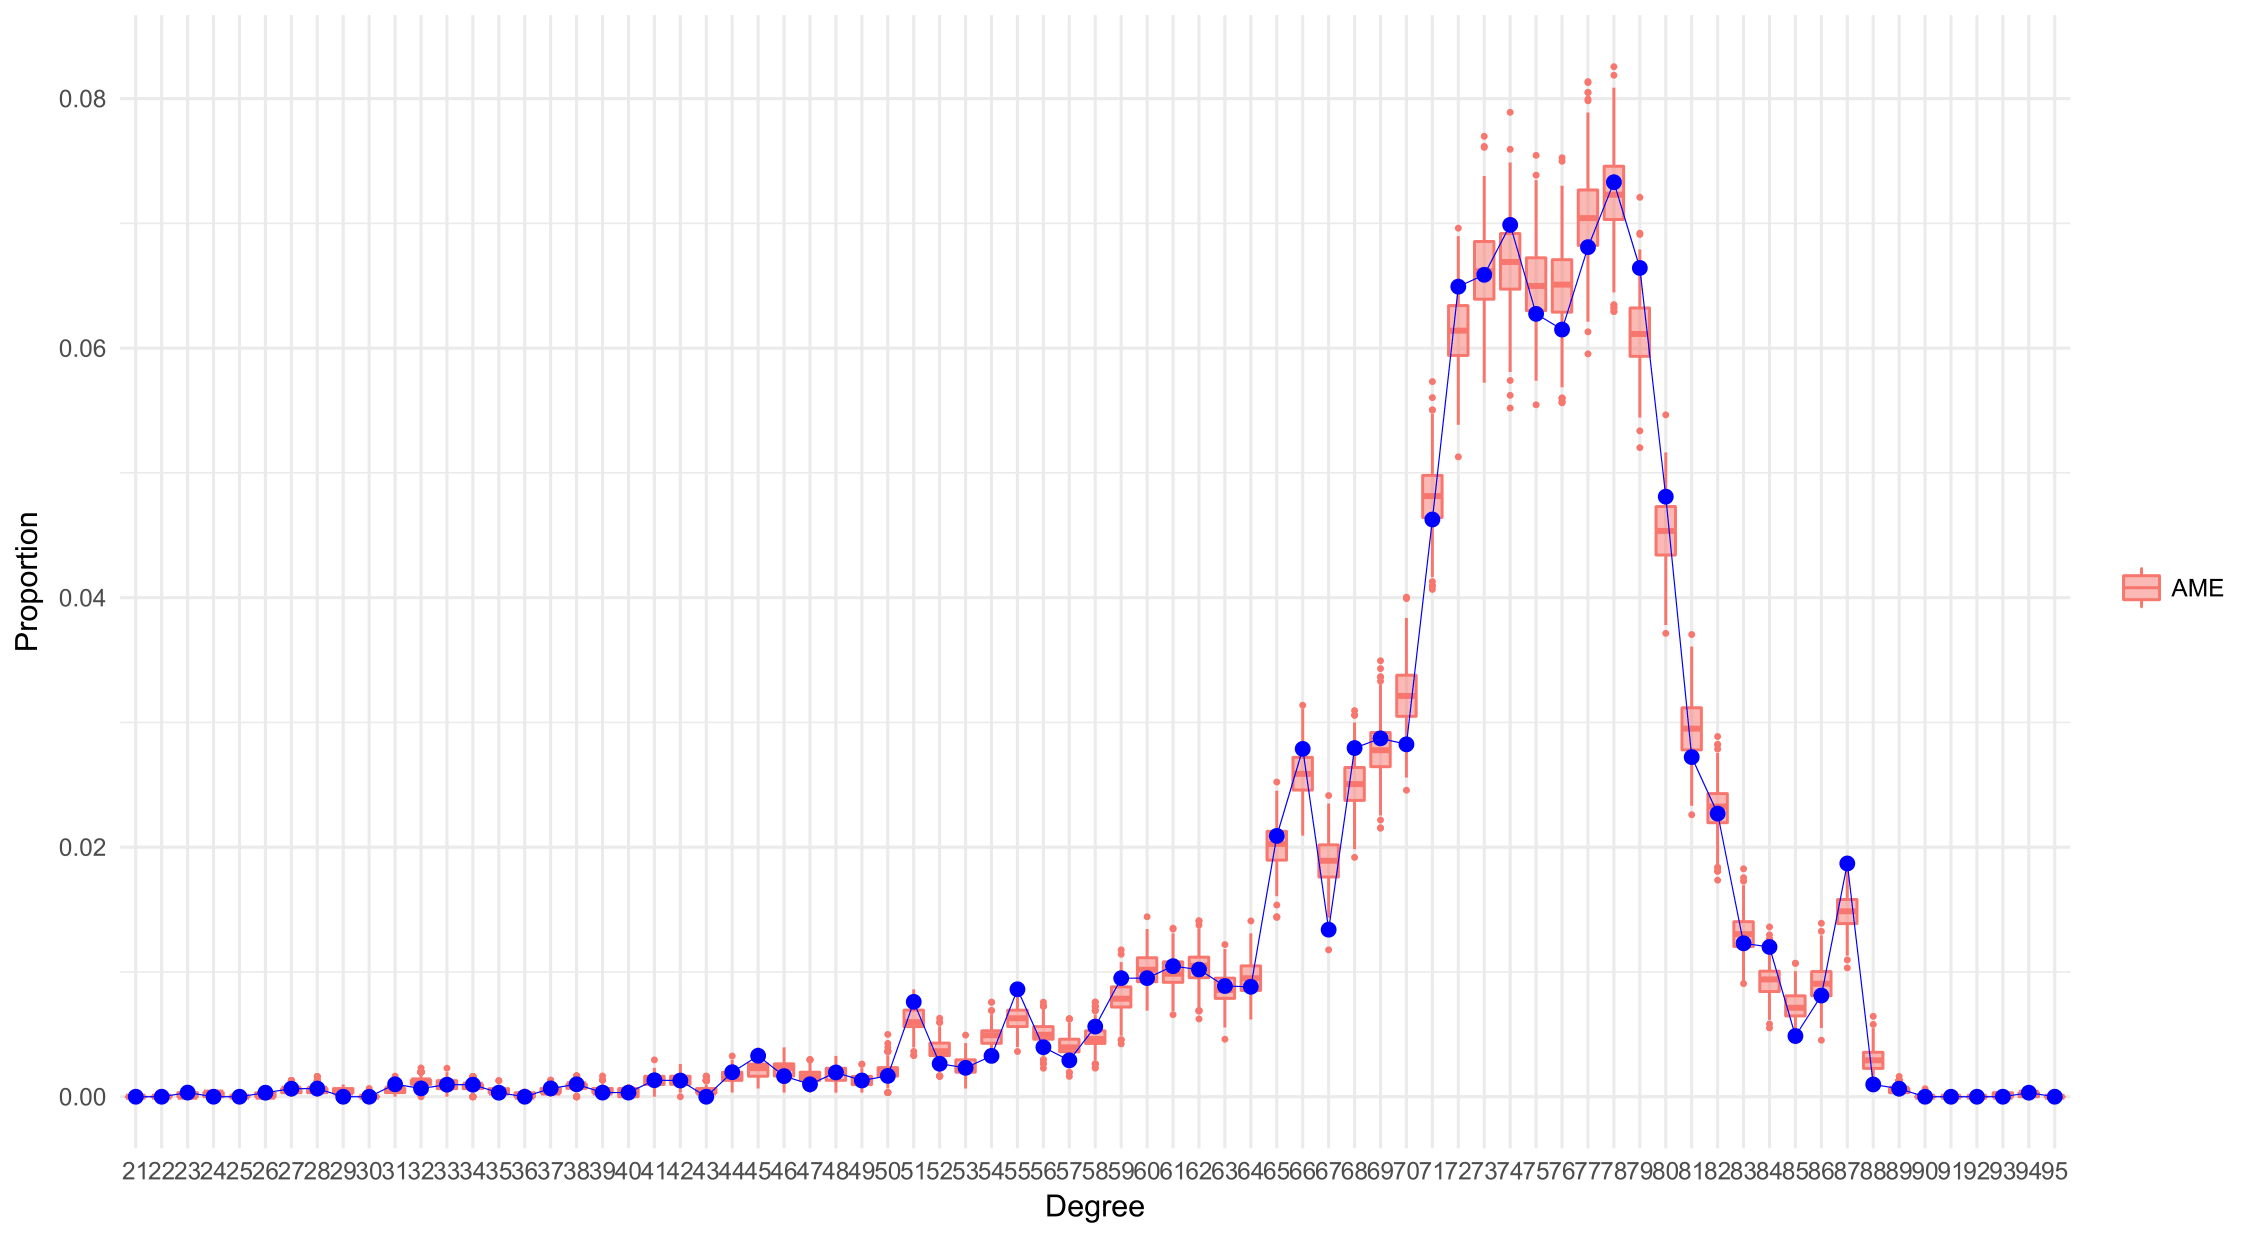
\includegraphics[width=0.64\textwidth]{plots_paper/AMEoveralldegree-1.png}	
			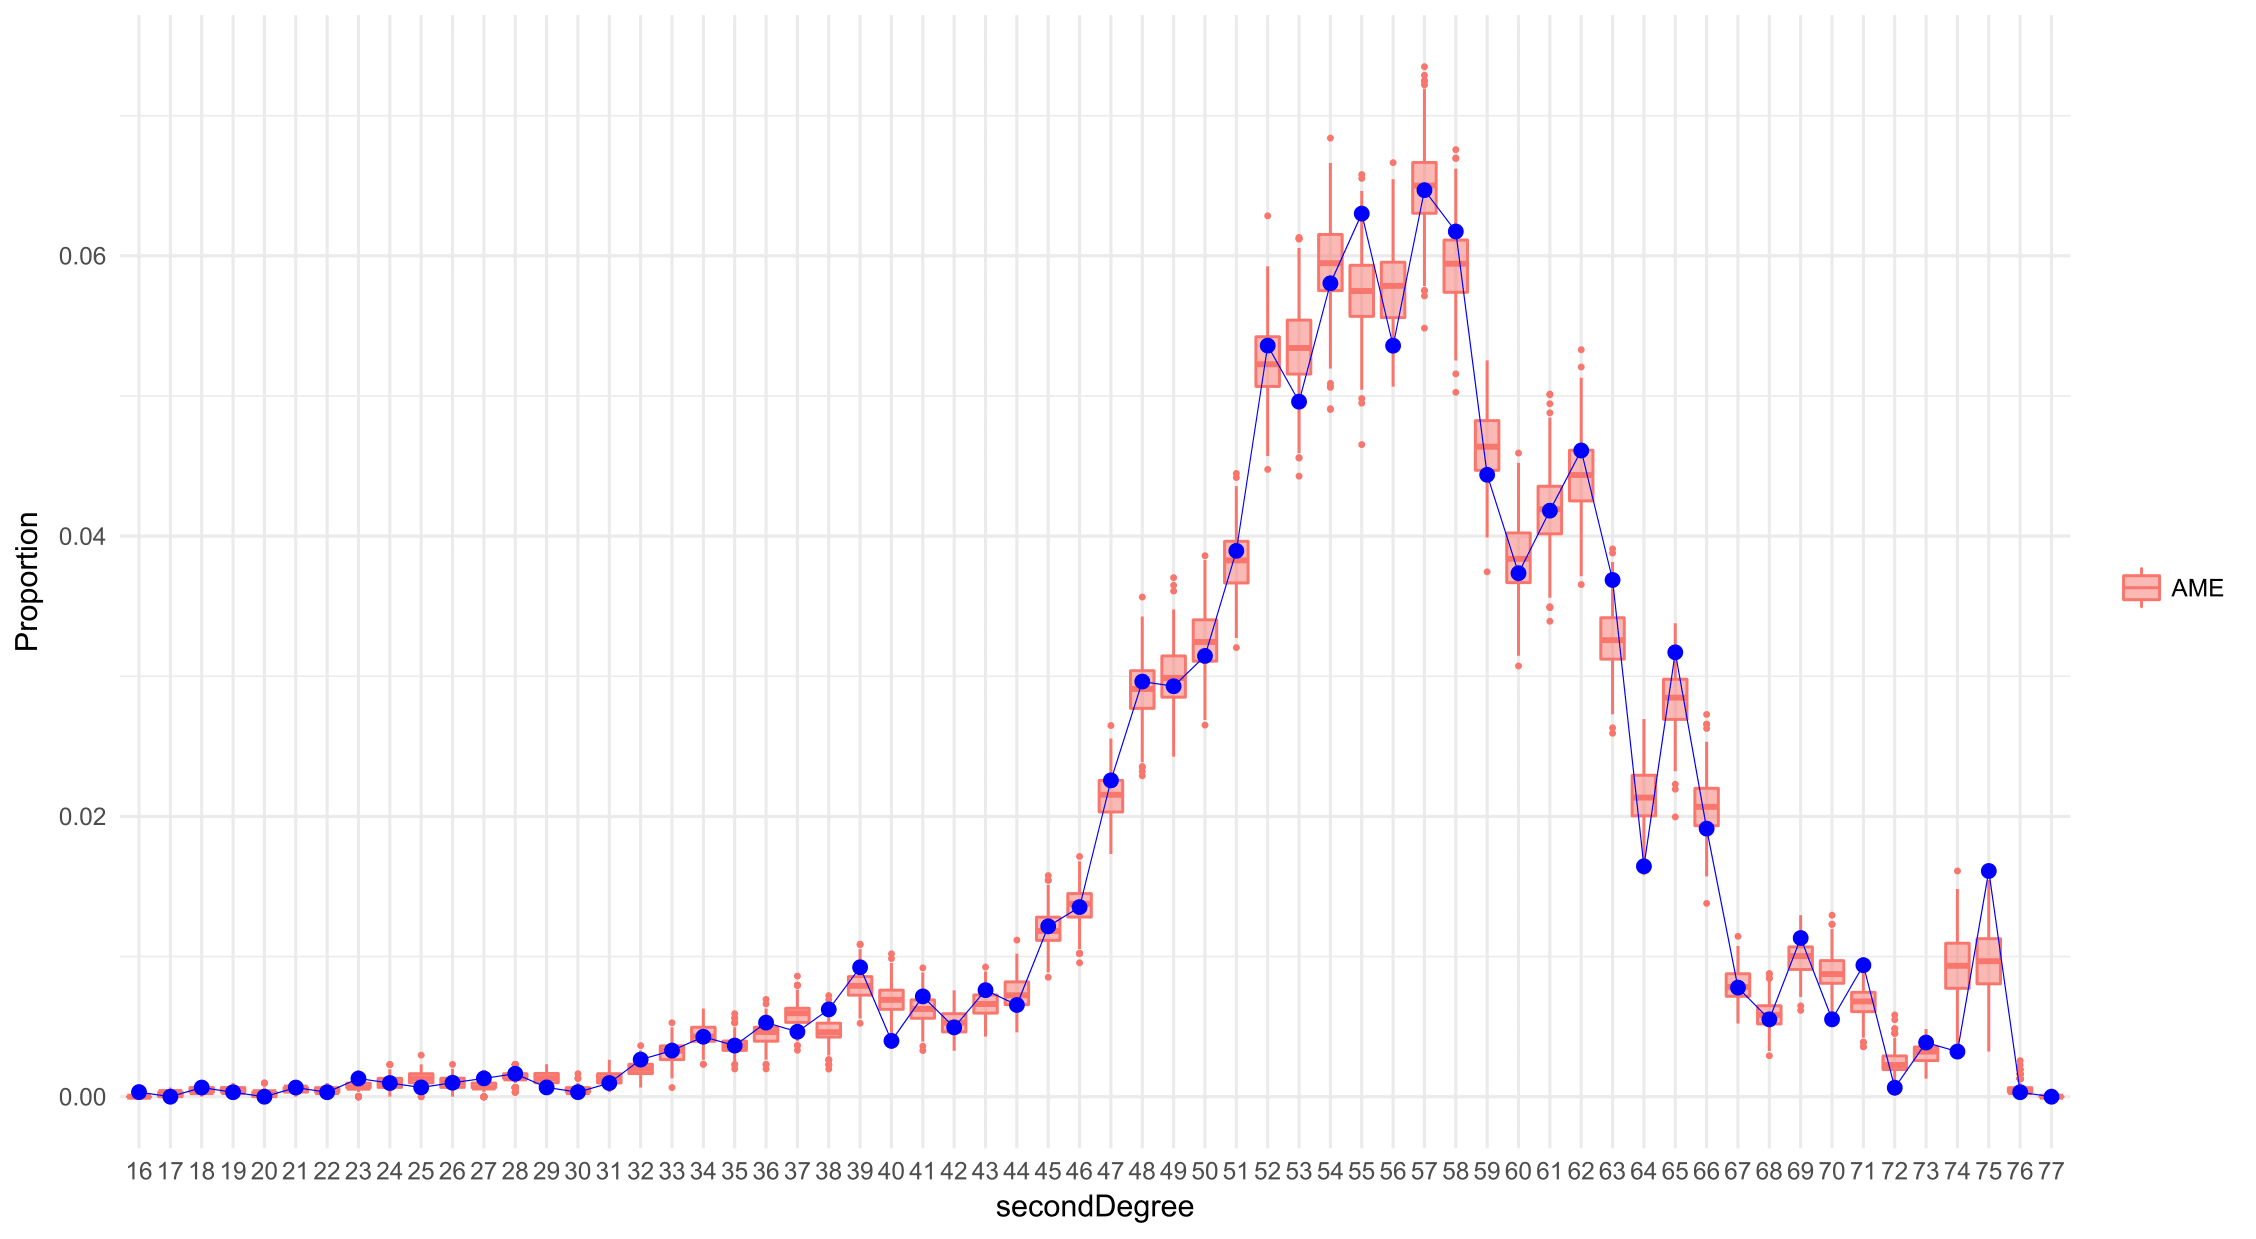
\includegraphics[width=0.64\textwidth]{plots_paper/AMEoverallsecond-1.png}
				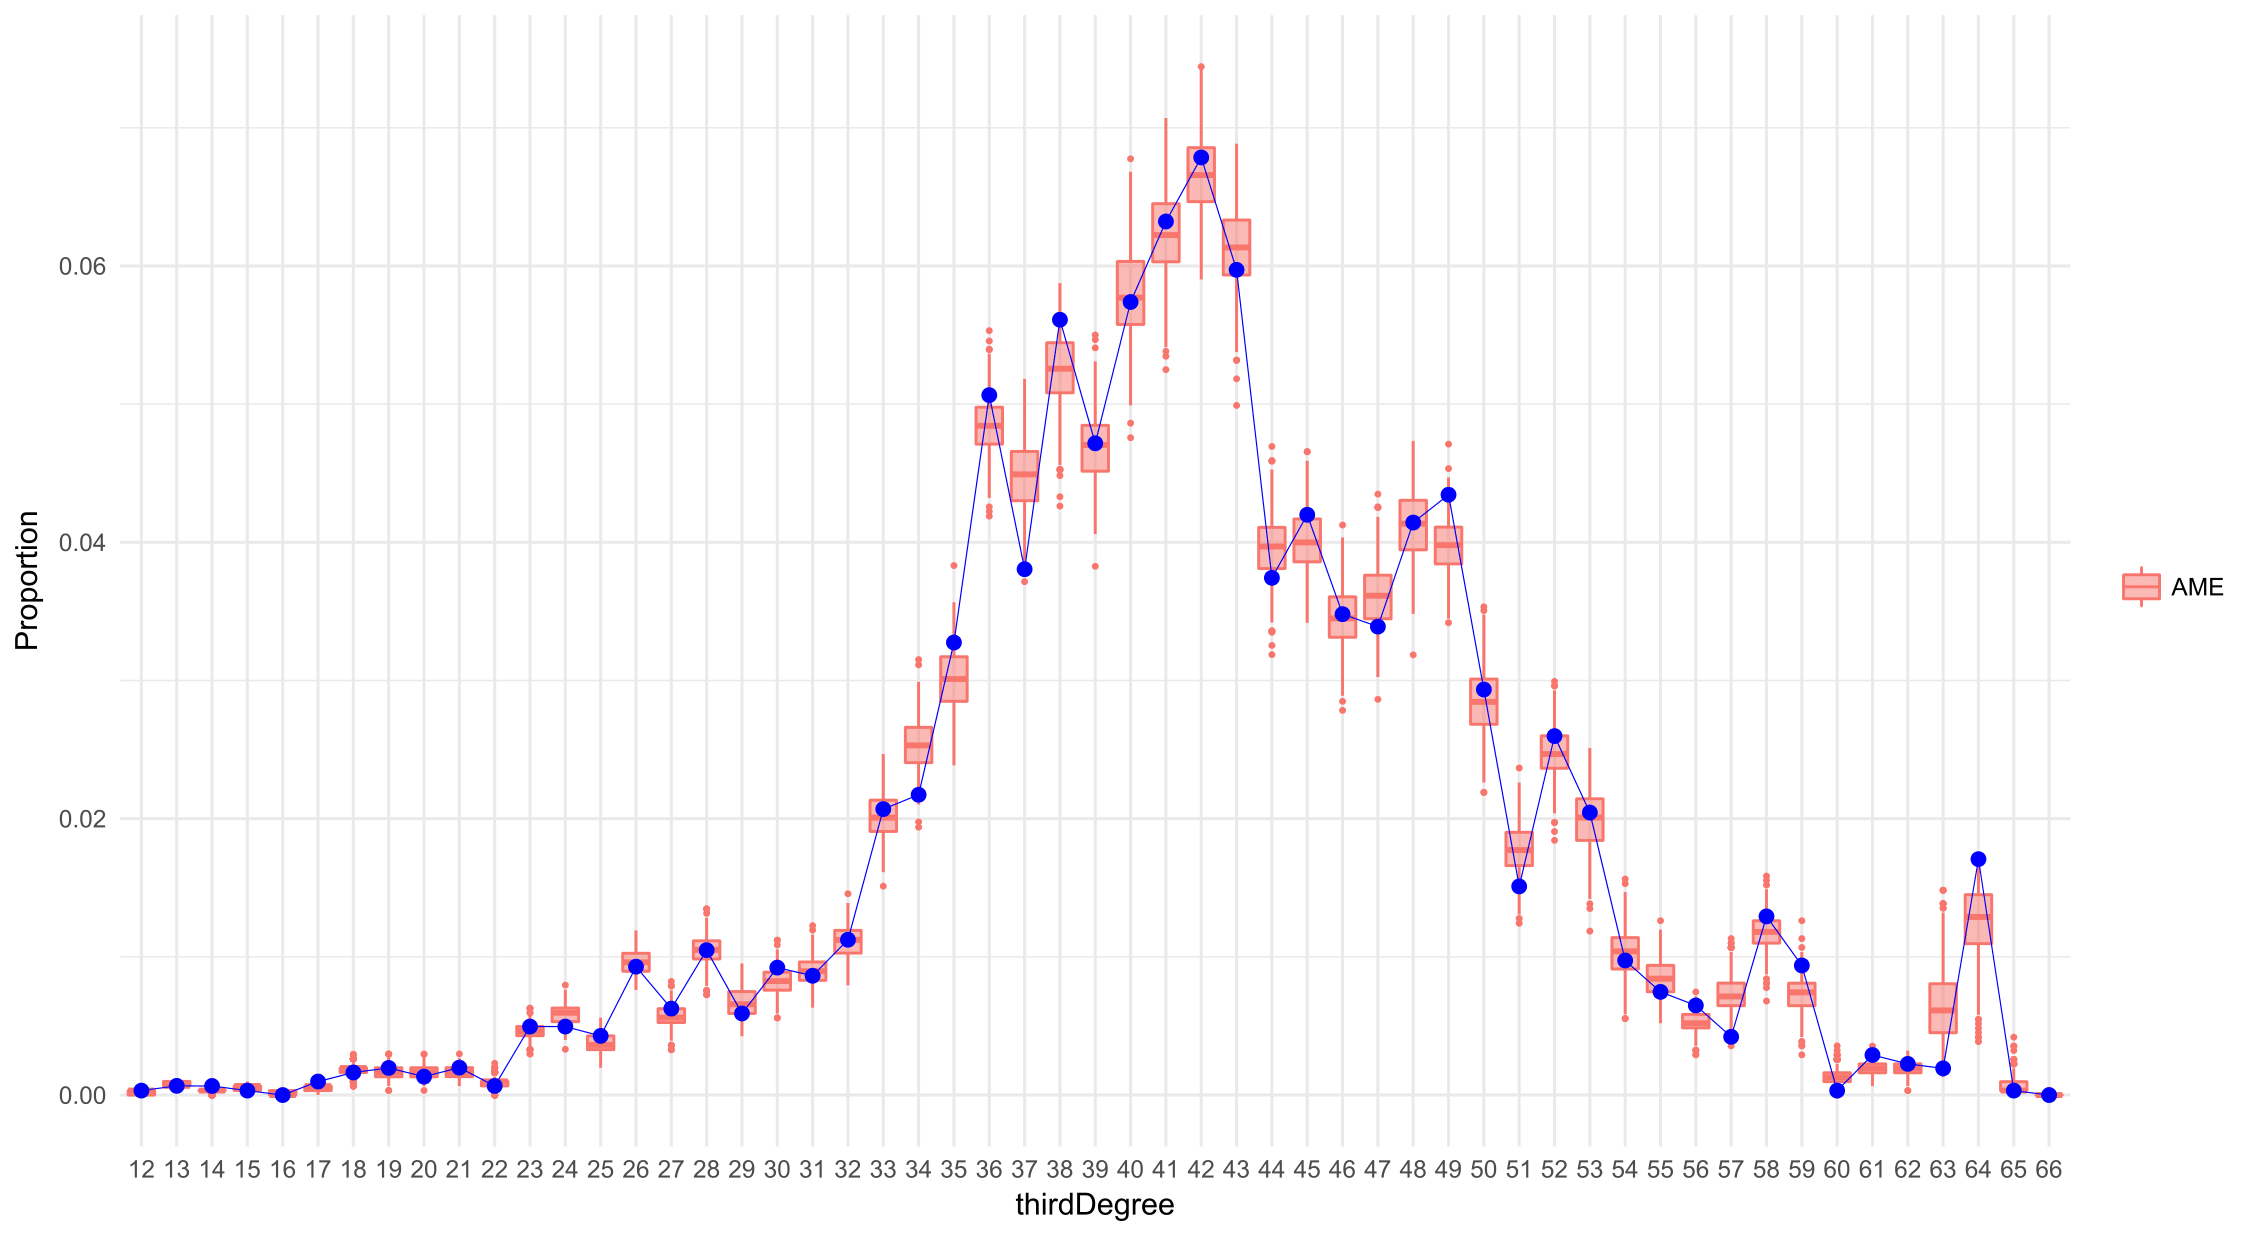
\includegraphics[width=0.64\textwidth]{plots_paper/AMEoverallthird-1.png}	
	\end{center}
\end{figure}

\end{appendices}
\end{document}

